% =====================================================================
% main.tex -- Geometry-aware neural operator surrogates for external aerodynamics
% =====================================================================
% Skeleton. Every section of the spec's section 11 outline, every one of the 12
% figures and 6 tables of spec section 8, each with a \label and a caption
% saying what will go there. Target 8-10 pages plus appendix.
%
% Build:  latexmk -pdf main.tex        (or: pdflatex, bibtex, pdflatex x2)
%
% Figures are drawn as framed placeholders by \figph so the document compiles
% before any figure exists. To drop in a real figure, delete the \figph line and
% uncomment the \includegraphics line above it. Numbers still awaiting a real
% run are wrapped in \pending{} (blue) and \todo{} (red); grep for both before
% submitting -- an accidental placeholder in a submitted paper is the kind of
% error that is remembered.
% =====================================================================
\documentclass[11pt,a4paper]{article}

\usepackage[utf8]{inputenc}
\usepackage[T1]{fontenc}
\usepackage[margin=1in]{geometry}
\usepackage{amsmath,amssymb,amsthm}
\usepackage{graphicx}
\usepackage{booktabs}
\usepackage{subcaption}
\usepackage{xcolor}
\usepackage[numbers,sort&compress]{natbib}
\usepackage[colorlinks=true,allcolors=blue]{hyperref}
\usepackage{siunitx}
\usepackage[expansion=false]{microtype}

\bibliographystyle{plainnat}

% =====================================================================
% macros.tex -- notation for the geometry-aware neural operator audit
% =====================================================================
% Notation matches section 5 of the project spec
% (../05_geometry_aware_neural_operator_surrogate_uq.md). If a symbol changes
% here it changes there too -- these macros are the single definition, so a
% reviewer can never be shown two spellings of the same quantity.
%
% Every symbol macro is wrapped in \ensuremath, so \FSC, \Rey, \Cd and friends
% typeset correctly in running text as well as inside $...$. Without that,
% writing "the FSC of \Mgnn" in a sentence is a compile error, which is exactly
% the kind of friction that ends with someone hard-coding \mathrm{FSC} in the
% body and the notation drifting apart.
%
% Naming convention: \*op for operators, \C* for coefficients, \Loss* for loss
% terms, \b* for bold vectors.
% =====================================================================

% ---------------------------------------------------------------------
% Vectors and general symbols
% ---------------------------------------------------------------------
\newcommand{\bx}{\ensuremath{\mathbf{x}}}
\newcommand{\by}{\ensuremath{\mathbf{y}}}
\newcommand{\bz}{\ensuremath{\mathbf{z}}}
\newcommand{\bn}{\ensuremath{\mathbf{n}}}                 % outward unit normal (into the fluid)
\newcommand{\bv}{\ensuremath{\mathbf{v}}}                 % velocity field
\newcommand{\bF}{\ensuremath{\mathbf{F}}}                 % integrated surface force
\newcommand{\btau}{\ensuremath{\boldsymbol{\tau}}}
\newcommand{\tauw}{\ensuremath{\btau_{w}}}                % wall shear stress vector
\newcommand{\eps}{\ensuremath{\varepsilon}}
\newcommand{\norm}[1]{\ensuremath{\left\lVert #1 \right\rVert}}
\newcommand{\abs}[1]{\ensuremath{\left\lvert #1 \right\rvert}}
\newcommand{\inner}[2]{\ensuremath{\left\langle #1, #2 \right\rangle}}
\newcommand{\R}{\ensuremath{\mathbb{R}}}
\newcommand{\Prob}{\ensuremath{\mathbb{P}}}
\newcommand{\Expect}{\ensuremath{\mathbb{E}}}
\newcommand{\indicator}{\ensuremath{\mathbb{1}}}
\newcommand{\degrees}{\ensuremath{^{\circ}}}              % NOT \degree: that name belongs to siunitx

% ---------------------------------------------------------------------
% Geometry and domain (spec 5.1)
% ---------------------------------------------------------------------
\newcommand{\geom}{\ensuremath{g}}                        % the geometry / shape
\newcommand{\dom}{\ensuremath{\Omega_{g}}}                % fluid domain exterior to the body
\newcommand{\bnd}{\ensuremath{\Gamma_{g}}}                % body surface
\newcommand{\cond}{\ensuremath{c}}                        % flow condition (U_inf, alpha)
\newcommand{\Uinf}{\ensuremath{U_{\infty}}}
\newcommand{\aoa}{\ensuremath{\alpha}}
\newcommand{\Rey}{\ensuremath{\mathrm{Re}}}
\newcommand{\chord}{\ensuremath{L}}
\newcommand{\Aref}{\ensuremath{A_{\text{ref}}}}
\newcommand{\einf}{\ensuremath{\mathbf{e}_{\infty}}}      % freestream unit direction
\newcommand{\eperp}{\ensuremath{\mathbf{e}_{\perp}}}      % lift direction, rot90(einf)
\newcommand{\sdf}{\ensuremath{s_{g}}}                     % signed distance function
\newcommand{\nut}{\ensuremath{\nu_t}}

% ---------------------------------------------------------------------
% The operator and its surrogate (spec 5.1)
% ---------------------------------------------------------------------
\newcommand{\Sop}{\ensuremath{\mathcal{S}}}               % true solution operator
\newcommand{\Sbnd}{\ensuremath{\mathcal{S}_{\Gamma}}}     % restricted to the surface trace
\newcommand{\Stheta}{\ensuremath{\mathcal{S}_{\theta}}}   % learned surrogate
\newcommand{\Kop}{\ensuremath{\mathcal{K}}}               % kernel-integral operator
\newcommand{\Pop}{\ensuremath{\mathcal{P}}}               % lifting
\newcommand{\Qop}{\ensuremath{\mathcal{Q}}}               % projection
\newcommand{\Fop}{\ensuremath{\mathcal{F}}}               % Fourier transform
\newcommand{\uhat}{\ensuremath{\hat{u}}}
\newcommand{\ubar}{\ensuremath{\bar{u}}}
\newcommand{\cp}{\ensuremath{c_p}}                        % surface pressure coefficient

% ---------------------------------------------------------------------
% Force integration and self-consistency (spec 5.4) -- the paper's core
% ---------------------------------------------------------------------
% Two independent routes to the same coefficient:
%   \Cdint / \Clint   : quadrature of the predicted surface fields
%   \Cdhead / \Clhead : direct regression head on the same backbone
% Their disagreement is the Force Self-Consistency, computable without labels.
\newcommand{\Cd}{\ensuremath{C_D}}
\newcommand{\Cl}{\ensuremath{C_L}}
\newcommand{\Cm}{\ensuremath{C_M}}
\newcommand{\Cdint}{\ensuremath{C_D^{\text{int}}}}
\newcommand{\Clint}{\ensuremath{C_L^{\text{int}}}}
\newcommand{\Cdhead}{\ensuremath{C_D^{\text{head}}}}
\newcommand{\Clhead}{\ensuremath{C_L^{\text{head}}}}
\newcommand{\Cdtrue}{\ensuremath{C_D^{\text{true}}}}
\newcommand{\Cltrue}{\ensuremath{C_L^{\text{true}}}}
\newcommand{\Cint}{\ensuremath{C^{\text{int}}}}
\newcommand{\Chead}{\ensuremath{C^{\text{head}}}}
\newcommand{\Ctrue}{\ensuremath{C^{\text{true}}}}
\newcommand{\FSC}{\ensuremath{\mathrm{FSC}}}
\newcommand{\FSCrel}{\ensuremath{\mathrm{FSC}_{\text{rel}}}}
\newcommand{\dS}{\ensuremath{\,\mathrm{d}S}}
\newcommand{\dmu}{\ensuremath{\,\mathrm{d}\mu}}

% ---------------------------------------------------------------------
% Losses (spec 5.3--5.5)
% ---------------------------------------------------------------------
\newcommand{\Loss}{\ensuremath{\mathcal{L}}}
\newcommand{\Lossdata}{\ensuremath{\mathcal{L}_{\text{data}}}}
\newcommand{\Lossforce}{\ensuremath{\mathcal{L}_{\text{force}}}}
\newcommand{\Lossbc}{\ensuremath{\mathcal{L}_{\text{bc}}}}     % no-slip
\newcommand{\Losssym}{\ensuremath{\mathcal{L}_{\text{sym}}}}   % symmetry / equivariance
\newcommand{\Lossdiv}{\ensuremath{\mathcal{L}_{\text{div}}}}   % divergence
\newcommand{\lamF}{\ensuremath{\lambda_F}}
\newcommand{\lamB}{\ensuremath{\lambda_B}}
\newcommand{\lamS}{\ensuremath{\lambda_S}}
\newcommand{\lamD}{\ensuremath{\lambda_D}}
\newcommand{\refl}{\ensuremath{R}}                             % reflection about the symmetry plane
\newcommand{\reflsharp}{\ensuremath{R^{\sharp}}}               % its action on vector fields

% ---------------------------------------------------------------------
% Ensembles, conformal prediction, calibration (spec 5.6)
% ---------------------------------------------------------------------
\newcommand{\nens}{\ensuremath{K}}
\newcommand{\sigmahat}{\ensuremath{\hat{\sigma}}}
\newcommand{\qhat}{\ensuremath{\hat{q}}}
\newcommand{\conf}{\ensuremath{\mathcal{C}_{\alpha}}}          % conformal interval
\newcommand{\Cov}{\ensuremath{\widehat{\mathrm{Cov}}}}
\newcommand{\ECE}{\ensuremath{\mathrm{ECE}}}
\newcommand{\nomlevel}{\ensuremath{1-\alpha}}
\newcommand{\score}{\ensuremath{s}}

% ---------------------------------------------------------------------
% Splits, shift and acquisition (spec 5.7--5.8)
% ---------------------------------------------------------------------
\newcommand{\shift}{\ensuremath{\Delta}}                       % shift magnitude: x-axis of the central figure
\newcommand{\acq}{\ensuremath{a}}                              % acquisition score
\newcommand{\betaacq}{\ensuremath{\beta}}
\newcommand{\gammaacq}{\ensuremath{\gamma}}
\newcommand{\splitname}[1]{\texttt{#1}}                        % \splitname{reynolds}, \splitname{shape5}, ...

% ---------------------------------------------------------------------
% Model shorthands, so the three architectures are never renamed mid-paper
% ---------------------------------------------------------------------
\newcommand{\Mgnn}{\textsc{M1-GNN}}
\newcommand{\Mfno}{\textsc{M2-SDF-FNO}}
\newcommand{\Mtrans}{\textsc{M3-Transolver}}

% ---------------------------------------------------------------------
% Drafting aids -- REMOVE every use of these before submission.
% \pending is deliberately NOT called \num: siunitx owns that name.
% ---------------------------------------------------------------------
\newcommand{\todo}[1]{\textcolor{red}{\textbf{[TODO: #1]}}}
\newcommand{\placeholder}[1]{\textcolor{gray}{\textit{[#1]}}}
\newcommand{\pending}[1]{\textcolor{blue}{#1}}   % a number still awaiting a real run


% Framed placeholder so the skeleton compiles with no figure files present.
\newcommand{\figph}[2][0.6\textwidth]{%
  \fbox{\parbox[c][0.22\textheight][c]{#1}{\centering\small\itshape\color{gray} #2}}}

\title{Geometry-Aware Neural Operator Surrogates for External Aerodynamics:\\
       Physics Consistency, Out-of-Distribution Generalization\\
       and Calibrated Uncertainty}
\author{T. Amin\thanks{Correspondence: \texttt{taimooramin419@gmail.com}. Code,
        split manifests, model cards and the Fluent verification set:
        \todo{repository URL}.}}
\date{\today}

\begin{document}
\maketitle

\begin{abstract}
Geometry-conditioned neural surrogates are reported as accurate on external
aerodynamics benchmarks, but almost always evaluated in one narrow sense: field
or drag error, in distribution, with no check on whether the prediction is
internally consistent or the reported uncertainty means anything. We audit three
geometry-conditioning families --- a $k$-nearest-neighbour graph network, a
signed-distance-conditioned Fourier neural operator in the GINO style, and a
Transolver-style geometry transformer, each reimplemented at matched parameter
count ($\sim$1.3--1.4\,M) and training budget --- under a single protocol built
around three deployment-relevant axes: force self-consistency, generalization
under six distribution shifts, and calibrated uncertainty. The central
instrument is force self-consistency (\FSC), the disagreement between the drag
obtained by quadrature of a model's own predicted surface pressure and the drag
from a regression head on the same backbone; \FSC{} needs no ground truth, so it
is computable out of distribution and on unlabelled candidate geometries. On
AirfRANS, with our force integrator gated against the dataset's own reported
coefficients (median relative error \pending{$3.3\times10^{-4}$}), three findings
recur across all three architectures: field accuracy separates the models
cleanly (transformer $>$ operator $>$ graph net, everywhere), but $C_D$ rank
correlation --- the quantity a designer actually uses --- does not: all three sit
at $\rho_s\approx$\pending{0.95--0.999}, closer to each other than to a plain
ridge-regression baseline on the shape and flow parameters ($\rho_s\approx$
\pending{0.83--0.90}), so the spread between splits dwarfs the spread between
models; and \FSC{} is smallest in distribution and largest under the hardest
(combined shape-and-Reynolds) shift for every architecture, typically growing
faster than the field error itself, making it a working label-free
out-of-distribution detector even though its growth between the intermediate
splits is not perfectly monotone.
Calibration (deep ensembles plus split conformal prediction), data-efficiency
curves, targeted ablations, and an uncertainty-driven active-learning loop
verified against independent Ansys Fluent simulations are designed into the same
protocol and reported as they land; this preprint states plainly which results
are complete and which are in progress. Code, split manifests, and model cards:
\todo{repository URL}.
\end{abstract}

% =====================================================================
\section{Introduction}
\label{sec:intro}
% =====================================================================

The external-aerodynamics surrogate literature has converged on a narrow
scoreboard: relative $L_2$ error on velocity and pressure fields, plus an error
or rank correlation on drag. Papers get accepted on that scoreboard. Engineers
cannot use it, for three reasons.

\textbf{Gap 1: internal inconsistency is invisible.} Models are trained with a
field loss and, sometimes, a separate head for integrated coefficients. Nothing
forces the predicted surface pressure and wall shear stress to integrate to the
predicted drag. A model can be accurate in field norm while being internally
inconsistent about the one number --- an integrated force coefficient --- a
designer actually acts on, because force is a small difference of large,
partially cancelling contributions dominated by regions (leading-edge suction
peak, separation onset, base pressure) that carry little weight in a
domain-averaged norm. That internal gap is a cheap, ground-truth-free diagnostic
almost nobody reports; we make it a first-class measurement.

\textbf{Gap 2: out-of-distribution failure is acknowledged but not
characterized.} Reported gains are almost always measured on random,
in-distribution splits, while deployment means new operating points and new
shapes. Prior benchmarking work states plainly that OOD generalization remains
a challenge for every method tested \citep{rabeh2025benchmarking} --- a
conclusion, not a characterization. Which axis of shift hurts most: Reynolds
number, angle of attack, or shape family? Does error grow smoothly or fail
discontinuously once separation appears? We evaluate on six splits spanning four
shift axes --- data scarcity, Reynolds number, angle of attack, and shape family
--- plus a fifth split that shifts shape and Reynolds together, the hardest
cell, and plot every metric against split identity and, where a numeric shift
magnitude $\shift$ is meaningful, against $\shift$ itself (\S\ref{sec:protocol}),
rather than reporting a single aggregate.

\textbf{Gap 3: uncertainty is reported without calibration.} Where uncertainty
is reported at all it is usually an ensemble spread: a heuristic score, least
trustworthy under exactly the shift where it matters, rarely checked against
realised coverage and almost never checked \emph{under shift}. Split conformal
prediction converts any such score into finite-sample coverage under
exchangeability --- a genuine guarantee in distribution, and a measurable
failure mode out of it --- yet conformal coverage for aerodynamic surface fields
and derived coefficients has not been systematically reported.

\paragraph{Contributions.}
\begin{enumerate}\itemsep2pt
  \item \textbf{C1: force self-consistency (\FSC)} as a label-free diagnostic,
        defined in \S\ref{sec:protocol} and evaluated on every split.
  \item \textbf{C2: a matched-budget audit} of three geometry-encoding families
        (graph, SDF-conditioned FNO, geometry transformer) under one protocol,
        one data pipeline and one training budget.
  \item \textbf{C3: calibration under shift}, deep ensembles plus split conformal
        prediction, with coverage reported against $\shift$ and the
        exchangeability assumption stated where it breaks.
  \item \textbf{C4: a solver-verified loop}, in which an acquisition score built
        from \FSC{} and ensemble spread selects candidate cases that are then run
        in Ansys Fluent, independent of the solver that generated the training
        data.
\end{enumerate}

\begin{figure}[t]
  \centering
  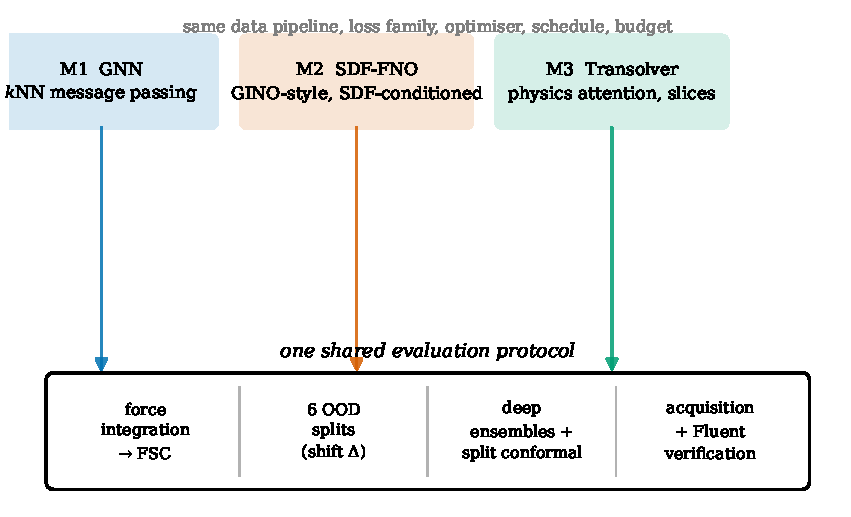
\includegraphics[width=0.92\textwidth]{figures/fig01_schematic.pdf}
  \caption{The three geometry-encoding families and the shared evaluation
           protocol beneath them: only the encoder changes; the force
           integration, the six OOD splits, the ensembling/conformal
           calibration and the acquisition/Fluent loop are identical across
           \Mgnn, \Mfno{} and \Mtrans.}
  \label{fig:schematic}
\end{figure}

% =====================================================================
\section{Related work}
\label{sec:related}
% =====================================================================

\paragraph{Neural operators and geometry encoding.}
Fourier neural operators \citep{li2021fno}, their geometry-informed extension
\citep{li2023gino}, and the general operator-learning framework
\citep{kovachki2023neuraloperator} together with DeepONet \citep{lu2021deeponet}
and mesh-based graph networks \citep{pfaff2021meshgraphnets} define the design
space. Transolver \citep{wu2024transolver} represents the attention-based branch.

\paragraph{Benchmarks for flow around complex geometry.}
AirfRANS \citep{bonnet2022airfrans} supplies the dataset, the metric definitions
and the Reynolds and angle-of-attack splits this study inherits.
\citet{rabeh2025benchmarking} is the closest prior art and the framing anchor: it
compares operators and foundation models across geometry encodings. Our axis is
consistency and calibration rather than an accuracy ranking, so we cite it as
motivation rather than as a competitor. DrivAerNet++ \citep{elrefaie2024drivaernetpp}
provides the 3D extension. \citet{takamoto2022pdebench} and
\citet{ohana2024thewell} set the benchmark-documentation conventions we follow.

\paragraph{Physics-consistency losses.}
Physics-informed operators \citep{li2021pino} penalise PDE residuals during
training. We use the same machinery diagnostically --- residuals are reported
whether or not they are penalised --- which is what separates a measurement from
a training trick.

\paragraph{Uncertainty quantification.}
Deep ensembles \citep{lakshminarayanan2017ensembles} for the predictive spread;
split conformal prediction \citep{angelopoulos2021gentle, vovk2005algorithmic,
lei2018distributionfree} for distribution-free intervals, with
\citet{romano2019cqr} as an alternative score. \citet{tibshirani2019covariateshift}
is why our shape-family results are framed as a documented failure of
exchangeability rather than as a bug.
\citet{vinuesa2022enhancing} frames the CFD-community reception.

% =====================================================================
\section{Problem setup and the consistency protocol}
\label{sec:protocol}
% =====================================================================

This section is the conceptual core of the paper: the shared operator-learning
formulation, the force-integration route to a coefficient, the consistency
diagnostic built from the gap between that route and a learned head, and the
shift axes along which every model is evaluated.

\subsection{Operator learning setup}
Let $\dom \subset \R^d$ be the fluid domain exterior to a body with boundary
$\bnd$, and let $\cond$ be the flow condition; for the airfoil case
$\cond = (\Uinf, \aoa)$ with $\Rey = \Uinf \chord / \nu$. We seek
\begin{equation}
  \Sop : (\geom, \cond) \longmapsto u = (\bv, p, \nut)\big|_{\dom},
\end{equation}
restricted in practice to the surface trace
$\Sbnd : (\geom,\cond) \mapsto (\cp, \tauw)\big|_{\bnd}$, since surface pressure
and wall shear stress are what forces depend on.

\subsection{Force integration}
With $\bn$ the outward normal and $\Delta S_i$ the facet measure taken from the
fixed input geometry,
\begin{equation}
  \bF = \oint_{\bnd} \left( -p\,\bn + \tauw \right) \dS
      \;\approx\; \sum_{i=1}^{N_f} \left( -p_i \bn_i + \tauw^{(i)} \right) \Delta S_i,
  \label{eq:force}
\end{equation}
\begin{equation}
  \Cdint = \frac{\bF \cdot \einf}{\tfrac12 \rho \Uinf^2 \Aref}, \qquad
  \Clint = \frac{\bF \cdot \eperp}{\tfrac12 \rho \Uinf^2 \Aref}.
\end{equation}
Because $\Delta S_i$ and $\bn_i$ come from the geometry and not from the
prediction, \eqref{eq:force} is \emph{linear} in the predicted surface fields and
differentiable, so it costs essentially nothing to evaluate or to backpropagate
through.

Nothing in this paper is interpretable unless this integrator reproduces the
dataset's own reported coefficients on ground-truth fields, so we gate on it
before any model result is reported: evaluated on all 1000 AirfRANS simulations,
the median relative error is \pending{$3.3\times10^{-4}$} on $\Cd$
(95th percentile $1.2\times10^{-3}$, maximum $1.6\times10^{-3}$) and
\pending{$4.8\times10^{-6}$} (median) on $\Cl$ --- roughly two orders of
magnitude inside the $1\%$ tolerance we set for this gate, and about two orders
of magnitude below the field errors reported in \S\ref{sec:results}. Every
downstream \FSC{} number therefore reflects the model, not the quadrature.

\subsection{Force self-consistency}
With $\Chead$ from a direct regression head on the same backbone,
\begin{equation}
  \FSC = \abs{\Cint - \Chead}, \qquad
  \FSCrel = \frac{\abs{\Cint - \Chead}}{\abs{\Ctrue} + \eps}.
\end{equation}
\FSC{} needs no ground truth. That is the whole point: it is computable on
out-of-distribution splits and on unlabelled proposed geometries, which is what
makes it usable inside the active-learning loop of \S\ref{sec:activelearning}.
When the force term is switched on during training (\S\ref{sec:models}, ablated
rather than default), it penalises all three disagreements symmetrically,
$\Lossforce = \abs{\Cint - \Ctrue} + \abs{\Chead - \Ctrue} + \abs{\Cint - \Chead}$,
so pulling either route toward the truth also pulls them toward each other.

\subsection{Symmetry, no-slip and divergence residuals}
With $\refl$ the reflection about the relevant plane and $\reflsharp$ its action
on vector fields, for $\refl\bnd = \bnd$ and a symmetric condition,
\begin{equation}
  \Losssym = \norm{\uhat(\geom,\cond) - \reflsharp \uhat(\refl \geom, \refl \cond)}_2
             \big/ \norm{\uhat(\geom,\cond)}_2 .
\end{equation}
We also check antisymmetry on a symmetric section at $\pm\aoa$:
$\Cl(-\aoa) \approx -\Cl(\aoa)$ and $\Cd(-\aoa) \approx \Cd(\aoa)$. Two further
residuals are defined identically for every model and reported whether or not
they are penalised. No-slip, with $\mathcal{N}_\delta$ the volume sample points
within $\delta$ of the wall and $\omega(x) = 1 - \mathrm{dist}(x,\bnd)/\delta$ a
linear falloff weight,
\begin{equation}
  \Lossbc = \frac{1}{\abs{\mathcal{N}_\delta}}
            \sum_{x \in \mathcal{N}_\delta} \norm{\hat{\bv}(x)}^2 \, \omega(x) .
\end{equation}
Divergence, by least-squares gradients on the point cloud (or finite differences
on M2's latent grid),
\begin{equation}
  \Lossdiv = \frac{1}{\abs{\mathcal{X}}} \sum_{x} \left(\nabla \cdot \hat{\bv}(x)\right)^2 .
\end{equation}
Every residual in this section --- \Losssym, the antisymmetry gap, \Lossbc{} and
\Lossdiv{} --- is computed and logged for every trained model regardless of
whether its $\lambda$ weight in \S\ref{sec:models} is zero, precisely so that a
residual reported as a diagnostic is never confused with one that was optimised
away.

\subsection{Shift magnitude}
Each split's test simulations are compared against \emph{that split's own}
training support along the numeric design axes $\Rey$, $\aoa$ and section
thickness. For axis $j$ with training range $[\ell_j, h_j]$ and population
standard deviation $\sigma_j$ (over that split's train $\cup$ test),
\begin{equation}
  \shift_j(x) = \max\!\left(0,\; \frac{x - h_j}{\sigma_j},\; \frac{\ell_j - x}{\sigma_j}\right),
\end{equation}
zero for a test point inside the training box and otherwise its distance in
units of that axis's own spread, so the axes are commensurable. Shape family is
categorical rather than metric (4-digit and 5-digit NACA sections are different
parameterisations), so it contributes a binary term, $\shift_{\text{shape}} = 1$
if the test simulation's series is absent from training, else $0$ --- one "unit"
of shift, on the same scale as one standard deviation of a numeric axis. The
per-simulation shift magnitude is the Euclidean norm over these terms,
$\shift = \big(\shift_{\Rey}^2 + \shift_{\aoa}^2 + \shift_{\text{thickness}}^2 +
\shift_{\text{shape}}^2\big)^{1/2}$, so a point in support on every axis scores
zero and \splitname{combined} --- shifted on two axes at once --- lands
furthest out by construction. Averaged over each split's test set, the realised
values are, in the order the splits are otherwise reported,
$\shift \approx \pending{0.00,\ 0.00,\ 0.42,\ 0.23,\ 1.00,\ 1.10}$ for
\splitname{full}, \splitname{scarce}, \splitname{reynolds}, \splitname{aoa},
\splitname{shape5} and \splitname{combined}. Note that this places
\splitname{reynolds} numerically further from training support than
\splitname{aoa}, even though \S\ref{sec:results_ood} finds AoA shift the more
damaging of the two --- a first hint that raw design-space distance and
model-relevant difficulty are not the same thing, since angle-of-attack shift
in this dataset crosses into a qualitatively new flow regime (separation) that
a Euclidean distance in design parameters cannot see. Figure~\ref{fig:error_vs_shift}
is the paper's central figure; at the current stage of the study it plots error
against split identity (ordered by $\shift$) rather than against the continuous
$\shift$ value itself, since aggregating per-simulation $\shift$ into a
per-panel continuous axis is deferred to a later revision.

% =====================================================================
\section{Models and training}
\label{sec:models}
% =====================================================================

We compare three geometry-encoding families under one matched protocol: the
same shared coefficient head, the same loss family, the same optimiser and
schedule, the same per-epoch checkpointing, and parameter counts held within
$\pm20\%$ of a 1.5\,M target, so that architecture is the only thing that
differs between runs. Realised counts are
\pending{1{,}389{,}637} (\Mgnn), \pending{1{,}373{,}605} (\Mfno) and
\pending{1{,}281{,}701} (\Mtrans) --- a $\pm8\%$ spread, tighter than the budget
requires.

\paragraph{\Mgnn: graph baseline.} $k$-nearest-neighbour ($k=16$) message
passing on the surface point cloud with node features $(\bx_i, \bn_i, \kappa_i,
\cond)$: position, outward normal, local (signed Menger) curvature, and the
broadcast flow condition.

\paragraph{\Mfno: SDF-conditioned FNO.} A GINO-style kernel encoder scatters
surface features onto a $64\times64$ regular latent grid conditioned on
$\sdf$, an FNO2d stack (16 Fourier modes, width 32) acts there, and a kernel
decoder queries back to arbitrary surface points \citep{li2023gino, li2021fno}.

\paragraph{\Mtrans: geometry transformer.} Transolver-style physics attention
\citep{wu2024transolver}: soft-assign $N$ points to $M=32$ slices across 4
attention layers at width 128, attend among slice tokens, scatter back, at cost
$\mathcal{O}(NM + M^2)$.

\paragraph{Reimplementation.} All three architectures are reimplemented from
the cited papers rather than run from the authors' released code. The target
hardware (a 4\,GB Pascal-generation laptop GPU, with training moved to a cloud
T4 once the study outgrew it) cannot reliably install the usual compiled
geometry-learning dependencies (PyTorch Geometric, \texttt{torch\_scatter},
\texttt{neuraloperator}) on this stack, so every graph, spectral-convolution and
slice-attention operator here is written in plain PyTorch. A reviewer should
not read any number in this paper as a reproduction of a published result:
the comparison that is meaningful is the \emph{within-study} one, matched by
construction across the three families, not an absolute comparison against the
architectures' original papers.

\paragraph{Training.} Adam with a cosine learning-rate schedule, initial
learning rate \pending{$10^{-3}$}, gradient-norm clipping at 1.0, batch size 16
for all three architectures (matched, not per-model tuned), 400 epochs, fp32
throughout (no mixed precision --- the Pascal-generation hardware has no
practical fp16 tensor-core path). Every run checkpoints every epoch and resumes
from its own last checkpoint, which is what makes training across
interruptible free-tier cloud sessions viable. Normalisation statistics
(inputs and targets) are computed from \emph{that split's own} training list
only, never from a shared global set and never from calibration or test data,
so no OOD split's test statistics can leak into training even indirectly
through the input scaling.

\paragraph{Objective.}
\begin{equation}
  \Loss = \Lossdata + \lamF \Lossforce + \lamB \Lossbc
        + \lamS \Losssym + \lamD \Lossdiv,
\end{equation}
each auxiliary term normalised by its value at initialisation. Defaults are
$\lamF = \lamB = \lamS = \lamD = 0$: the physics terms are ablation flags, not
part of the headline models.

% =====================================================================
\section{Datasets and splits}
\label{sec:data}
% =====================================================================

AirfRANS \citep{bonnet2022airfrans}: 1000 steady incompressible RANS solutions
(Spalart--Allmaras) over NACA 4- and 5-digit sections, roughly 32{,}000 volume
mesh points and $O(10^3)$ surface points per case, $\Rey \in [2,6]\times 10^6$,
$\aoa \in [-5\degrees, +15\degrees]$, licensed \textbf{ODbL-1.0} (attribution and
share-alike on derived databases; we release split manifests and code, never a
processed copy of the fields). Every simulation encodes its own design point
(inlet velocity, angle of attack, NACA parameters) in its filename, which is
what makes the shift-magnitude computation of \S\ref{sec:protocol} and the new
splits below possible without any additional metadata.

DrivAerNet++ \citep{elrefaie2024drivaernetpp}, licensed \textbf{CC~BY-NC~4.0},
is this study's designated 3D extension --- surface pressure and drag on
$O(8000)$ car designs across fastback, notchback and estateback families --- but
it requires an interactive Globus authentication step outside this project's
current scope and is not part of any result reported here. \todo{Run and report
only if the 3D leg lands before submission; otherwise state explicitly in the
limitations that the paper is AirfRANS-only and DrivAerNet++ remains future
work, per the project's own scoping decision (results should never imply a 3D
leg that was not executed).}

\paragraph{Splits.} Six splits, all derived deterministically from the dataset's
own manifest or from parsed design parameters, each with train/calibration/test
lists that are asserted programmatically disjoint
(\texttt{tests/test\_splits\_no\_leakage.py}): in-distribution \splitname{full}
(the official random 800/200 train/test task); \splitname{scarce} (the official
low-data task, 200 training cases, evaluated on \splitname{full}'s test set,
which has no test set of its own); Reynolds shift \splitname{reynolds} (train
$\Rey\in[3,5]\times10^6$, test outside that band); angle-of-attack shift
\splitname{aoa} (train $\aoa\in[-2.5\degrees,12.5\degrees]$, test outside,
crossing into separation for the highest angles --- \todo{the pre-stall /
post-stall breakout by a wall-shear sign-change indicator is designed but not
yet computed per-simulation; currently \splitname{aoa} is reported as one
pooled test set}); shape-family shift \splitname{shape5} (train every NACA
4-digit simulation, test every 5-digit one, a family AirfRANS itself does not
split on); and \splitname{combined} (train 4-digit \emph{and} inside the
Reynolds training band, test 5-digit \emph{and} outside it --- shape and
Reynolds shifted together, the hardest cell, by design a strict strengthening
of \splitname{reynolds}). Calibration sets are the last $\min(100,
\max(1,\lceil 0.2\,n_{\text{train}}\rceil))$ entries of each split's own
seed-0-shuffled training list, so they scale with the split and never overlap
train or test; test is never touched by normalisation or calibration
(\S\ref{sec:models}).

\begin{table}[t]
  \centering
  \caption{\textbf{Table 6.} Dataset and split card: per-split sizes for train,
    calibration and test, mean shift magnitude $\shift$ over the test set
    (\S\ref{sec:protocol}), source dataset, and licence.}
  \label{tab:datacard}
  \begin{tabular}{lrrrlll}
    \toprule
    Split & Train & Cal & Test & $\bar\shift$ & Source & Licence \\
    \midrule
    \splitname{full}     & 700 & 100 & 200 & 0.00 & AirfRANS & ODbL-1.0 \\
    \splitname{scarce}   & 160 & 40  & 200 & 0.00 & AirfRANS & ODbL-1.0 \\
    \splitname{reynolds} & 404 & 100 & 496 & 0.42 & AirfRANS & ODbL-1.0 \\
    \splitname{aoa}      & 704 & 100 & 196 & 0.23 & AirfRANS & ODbL-1.0 \\
    \splitname{shape5}   & 391 & 98  & 511 & 1.00 & AirfRANS & ODbL-1.0 \\
    \splitname{combined} & 191 & 48  & 246 & 1.10 & AirfRANS & ODbL-1.0 \\
    \bottomrule
  \end{tabular}
\end{table}

% =====================================================================
\section{Results}
\label{sec:results}
% =====================================================================

\subsection{In-distribution}
\label{sec:results_id}

On the in-distribution split \splitname{full}, all three architectures are
accurate and closely spaced (Table~\ref{tab:indist}): field relative $L_2$ on
surface pressure ranges only from \pending{0.017} (\Mtrans) to \pending{0.074}
(\Mgnn), a $4.3\times$ span, while every model separates \Mgnn{} from the two
better encodings by a wider margin than any of the OOD splits separate the
architectures from each other (\S\ref{sec:results_ood}). The ordering is clean
and holds throughout the study: \Mtrans{} $>$ \Mfno{} $>$ \Mgnn{} on field
accuracy, everywhere, matching the operator-learning literature's expectation
that attention over learned slices and spectral mixing on a regular grid both
out-resolve local $k$NN message passing at matched budget. On $\Cd$ rank
correlation --- the quantity a designer actually uses for down-selection --- the
picture inverts: all three sit at $\rho_s = 0.999$ on \splitname{full}, a gap of
three parts per thousand between the best and worst architecture. The
\textbf{ridge baseline}, a linear regression from the shape and flow parameters
directly to $\Cd$ with 29 parameters and zero training cost, is reported
honestly rather than hidden: it reaches $\rho_s = 0.902$ in distribution ---
worse than every neural model, but far from a naive floor, and (as
\S\ref{sec:results_ood} shows) it holds up strikingly well under shift. All
three architectures also show a large, roughly uniform symmetry residual
(\pending{4.4--4.7}, Table~\ref{tab:indist}) --- consistent with the expectation
that none of these encodings is architecturally equivariant to reflection; none
uses the symmetry loss or augmentation during the runs reported here
(\S\ref{sec:models}), so this is the raw, unmitigated residual, and
Figure~\ref{fig:symmetry}/Table~\ref{tab:ablations} (\S\ref{sec:results_ablations})
is where an augmentation ablation would show whether it can be trained away.

\begin{table}[t]
\centering
\caption{In-distribution accuracy, consistency and cost (AirfRANS \texttt{full}).}
\label{tab:indist}
\begin{tabular}{lrrrrrrr}
\toprule
model & $p$ rel-$L_2$ & $\tau_w$ rel-$L_2$ & $C_D$ MAE & $C_D$ $\rho$ & FSC $C_D$ & sym & GPU-h \\
\midrule
M1 GNN & 0.0753 $\pm$ 0.00271 & 0.0686 $\pm$ 0.00212 & \textbf{0.000132 $\pm$ 1.5e-05} & 0.996 $\pm$ 0.00337 & 0.00539 $\pm$ 8.8e-05 & 4.47 $\pm$ 0.0268 & 2.88 $\pm$ 0.438 \\
M2 SDF-FNO & 0.0259 $\pm$ 0.00128 & 0.0307 $\pm$ 0.000882 & 0.000142 $\pm$ 1.26e-05 & 0.998 $\pm$ 0.000497 & 0.00162 $\pm$ 0.000195 & 4.51 $\pm$ 0.127 & 0.36 $\pm$ 0.00215 \\
M3 Transolver & \textbf{0.0186 $\pm$ 0.000933} & \textbf{0.0192 $\pm$ 0.000811} & 0.000135 $\pm$ 1.35e-05 & \textbf{0.999 $\pm$ 0.000359} & \textbf{0.00129 $\pm$ 0.000311} & 4.47 $\pm$ 0.0731 & 0.408 $\pm$ 0.000758 \\
Ridge & 1.42 & 1.16 & 0.0016 & 0.902 & 0.00604 & \textbf{0} & \textbf{0} \\
Constant & 1.42 & 1.16 & 0.00342 & -- & 0.0063 & \textbf{0} & \textbf{0} \\
\bottomrule
\end{tabular}
\end{table}


\begin{figure}[t]
  \centering
  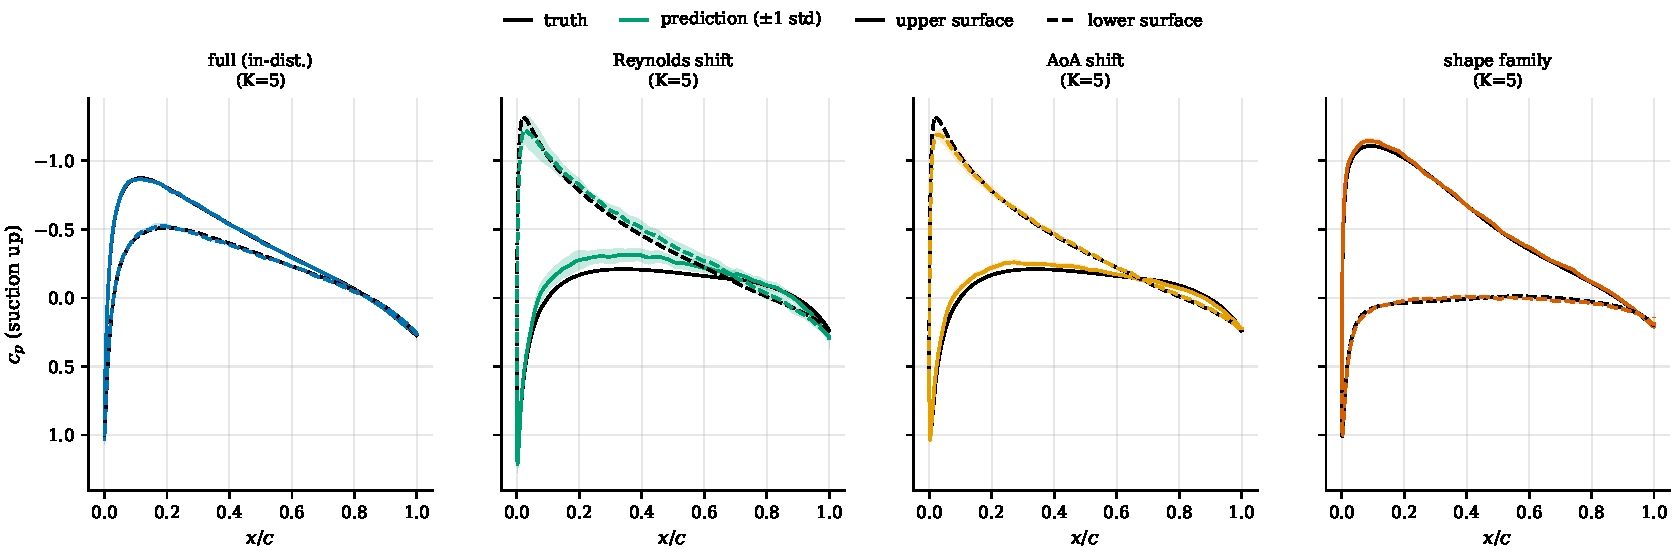
\includegraphics[width=\textwidth]{figures/fig02_cp_profiles.pdf}
  \caption{\Mtrans{} surface $\cp$, prediction versus truth, on one
           representative test simulation per split (full, Reynolds shift,
           AoA shift, shape family), upper and lower surface shown separately
           (solid/dashed), $\cp$ axis inverted (suction up, the aerodynamics
           convention). The shaded band is the $K=5$ deep-ensemble
           $\pm 1$ standard deviation. In distribution the ensemble mean is
           visually indistinguishable from truth and the band is a hairline;
           under Reynolds and AoA shift the mean develops a systematic
           offset near the suction peak and the band widens but --- exactly
           the pattern behind \S\ref{sec:results_calibration}'s coverage
           collapse --- not enough to keep the truth curve inside it; under
           shape-family shift (a new NACA digit family, same flow regime) the
           fit stays close and the band stays narrow, consistent with
           \splitname{shape5} being the mildest single-axis shift for every
           architecture (\S\ref{sec:results_ood}).}
  \label{fig:cp_profiles}
\end{figure}

\begin{figure}[t]
  \centering
  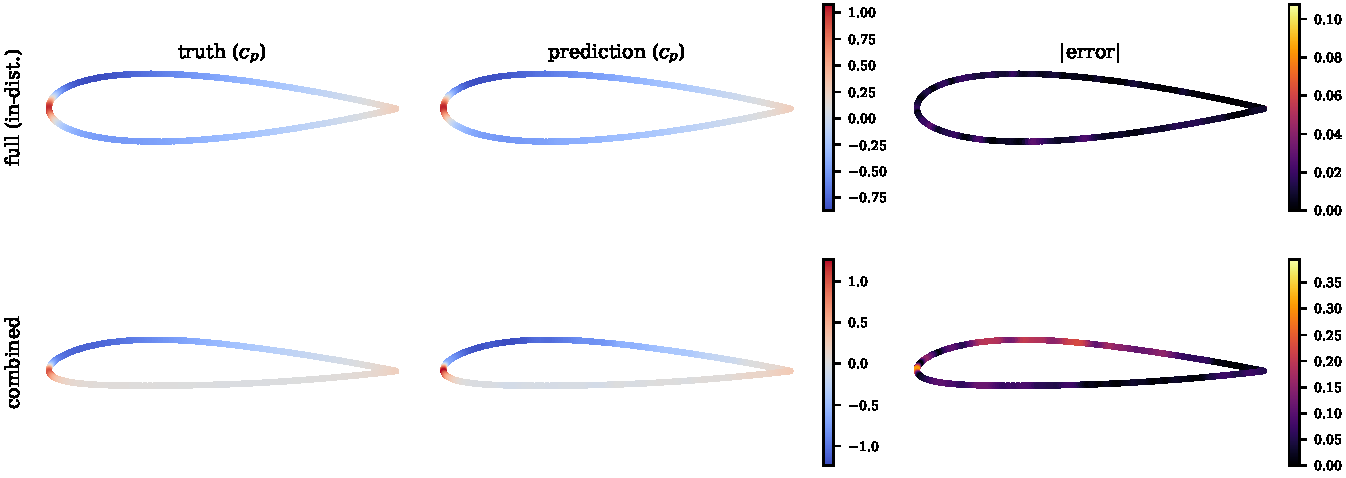
\includegraphics[width=\textwidth]{figures/fig03_surface_fields.pdf}
  \caption{\Mtrans{} surface $\cp$ scattered on the airfoil contour --- truth,
           prediction, and absolute error, shared colour scale on the first
           two panels per row --- for one in-distribution simulation
           (\splitname{full}) and one on the hardest shift
           (\splitname{combined}, shape and Reynolds shifted together), seed
           0. This panel replaces the three-DrivAerNet++-cars figure planned
           in the original design doc: DrivAerNet++ is out of scope for this
           preprint (\S\ref{sec:data}), so the "surface field" slot is filled
           with a second, complementary view of the same AirfRANS airfoils
           Figure~\ref{fig:cp_profiles} plots as a profile --- here the error
           is visibly concentrated near the leading edge, where the
           combined-shift suction peak is most mispredicted.}
  \label{fig:car_surfaces}
\end{figure}

\subsection{Out-of-distribution}
\label{sec:results_ood}

Figure~\ref{fig:error_vs_shift} and Table~\ref{tab:ood} give the full
$3\times6$ grid (three models, six splits). The hierarchy is consistent and
physical at the extremes, for every architecture: \splitname{full} is easiest
and \splitname{combined} is hardest, and \splitname{shape5} and
\splitname{scarce} sit as the two mildest single-axis shifts, in that order.
The two remaining single-axis shifts, \splitname{reynolds} and \splitname{aoa},
are consistently the two \emph{hardest} single-axis splits but do not settle
into one fixed order between them: \Mfno{} and \Mtrans{} both find
\splitname{aoa} harder than \splitname{reynolds}, while \Mgnn{} finds the
reverse. We report this rather than round it into a clean ranking --- it is a
genuine architecture-dependent disagreement on which axis hurts more, sitting
inside an otherwise architecture-independent hierarchy. \Mtrans{} degrades from
$0.017$ (\splitname{full}) to $0.139$ (\splitname{combined}), an
$8\times$ increase; \Mgnn{} degrades from $0.074$ to $0.270$, only $3.7\times$
--- the weaker in-distribution model is, in relative terms, \emph{more} robust
to shift, so ranking by in-distribution accuracy alone would misorder the
architectures for a deployment that includes shift. Notably this field-error
ordering does not track the shift-magnitude ordering of \S\ref{sec:protocol}:
\splitname{reynolds} and \splitname{aoa} ($\bar\shift = 0.42$ and $0.23$) are
the two hardest single-axis splits for every model, yet \splitname{shape5}
carries the single largest per-axis $\shift$ in the whole study ($\bar\shift =
1.00$, by construction --- any 5-digit test case counts as one full "unit" of
shift) while being the \emph{mildest} single-axis shift for every model. A
purely geometric shift measure and the models' actual difficulty ranking
disagree, and the natural explanation is physical rather than statistical:
$\aoa$ and $\Rey$ shift move the flow into conditions --- higher effective
angle of attack, different boundary-layer character --- that can cross into a
qualitatively new regime (separation), whereas a new NACA digit family at the
same $\Rey$ and $\aoa$ is still an attached-flow problem the model has seen the
physics of, just not the exact shape. That is consistent with the design doc's
hypothesis: these models interpolate within a flow regime and degrade
gracefully doing so, but degrade sharply once the physics itself changes
character, a regime change that a Euclidean distance in design parameters
cannot see. \todo{The pre-stall/post-stall breakout inside \splitname{aoa}
(\S\ref{sec:data}) would make this claim precise rather than inferred;
currently it rests on the aggregate \splitname{aoa}/\splitname{reynolds}
numbers and the domain knowledge that the \splitname{aoa} test range crosses
$\alpha\approx12$--$15\degrees$, close to typical NACA-section stall onset at
these Reynolds numbers.}
On $\Cd$ rank correlation the between-model gap stays under \pending{0.01} on
every split while the between-split gap for a single model reaches
\pending{0.05} (\Mgnn{}: $0.999\to0.945$); architecture matters an order of
magnitude less than shift for the metric a designer would actually use to
compare candidate shapes. The ridge baseline
is, again, the uncomfortable honest number: $\rho_s\in[0.83,0.90]$ across all
six splits (Table~\ref{tab:datacard}'s row order), meaning a 29-parameter
linear model captures most of the $\Cd$-ranking signal that these
$\sim$1.3\,M-parameter neural operators do, and the neural models' advantage on
ranking specifically (as opposed to field accuracy) is a few percentage points,
not the qualitative gap the field-error numbers suggest.

\begin{figure}[t]
  \centering
  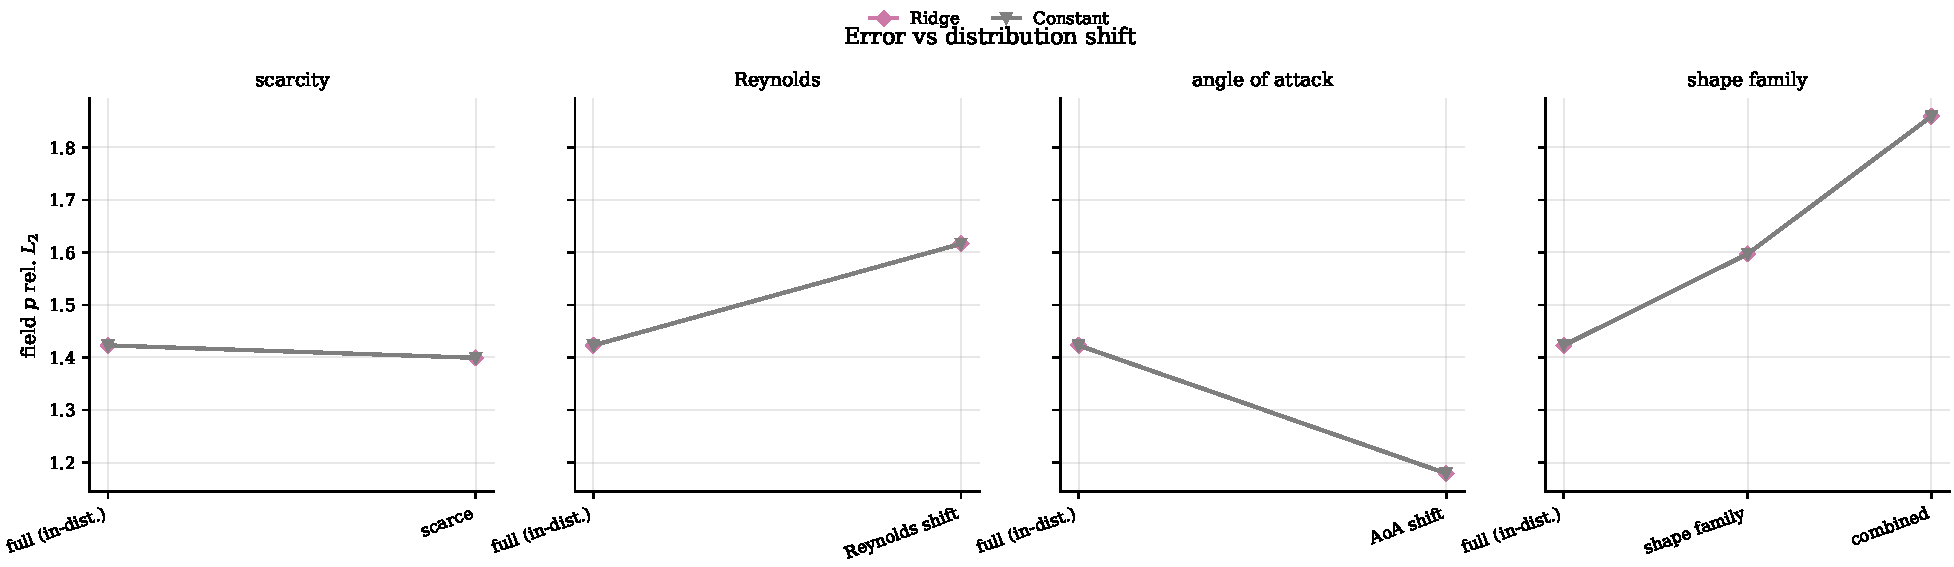
\includegraphics[width=\textwidth]{figures/fig04_error_vs_shift.pdf}
  \caption{Error versus distribution shift, one panel per OOD axis (scarcity,
           Reynolds, angle of attack, shape family/combined), one line per
           model, splits ordered along each axis. Field relative $L_2$ on
           surface pressure; the axis with the numeric shift magnitude
           $\shift$ from \S\ref{sec:protocol} is discussed in the text.}
  \label{fig:error_vs_shift}
\end{figure}

\begin{table}[t]
\centering
\caption{Out-of-distribution field $p$ rel-$L_2$ by split.}
\label{tab:ood}
\begin{tabular}{lrrrrrr}
\toprule
model & full (in-dist.) & scarce & Reynolds shift & AoA shift & shape family & combined \\
\midrule
M1 GNN & 0.0737 & 0.154 & 0.223 & 0.188 & 0.13 & 0.27 \\
M2 SDF-FNO & 0.0257 & 0.0832 & 0.0979 & 0.111 & 0.0641 & 0.153 \\
M3 Transolver & \textbf{0.0174} & \textbf{0.0666} & \textbf{0.0773} & \textbf{0.109} & \textbf{0.0546} & \textbf{0.139} \\
Ridge & 1.42 & 1.4 & 1.62 & 1.18 & 1.6 & 1.86 \\
Constant & 1.42 & 1.4 & 1.62 & 1.18 & 1.6 & 1.86 \\
\bottomrule
\end{tabular}
\end{table}


\subsection{Consistency}
\label{sec:results_consistency}

Pooled across all 18 (model, split) cells, \FSCrel{} on $\Cd$ correlates
strongly with field relative $L_2$ (Pearson $r=\pending{0.94}$, Spearman
$\rho=\pending{0.89}$): both quantities respond to the same underlying cause,
distribution shift, so a model that is doing worse on the field overall tends
also to be less self-consistent. That pooled correlation, however, is mostly a
statement about shift, not about the models: it is driven by both quantities
moving together as the split changes, not by consistency and field accuracy
agreeing about which \emph{architecture} is best on a fixed split. Holding the
split fixed, \Mtrans{} is both the most accurate and the most self-consistent
model on \splitname{full}, \splitname{scarce}, \splitname{shape5} and
\splitname{combined} --- but on the two hardest single-axis splits,
\splitname{reynolds} and \splitname{aoa}, \Mfno{} is \emph{more}
self-consistent than \Mtrans{} even though \Mtrans{} remains the more accurate
model in field norm. That is a concrete instance of the hypothesis this metric
is meant to test: the field-error leaderboard and the consistency leaderboard
disagree, and they disagree specifically on the two splits where it would
matter most to a designer relying on the field-best model's reported drag.
\FSCrel{} also grows faster than field error from \splitname{full} to
\splitname{combined} for two of the three architectures (\Mgnn:
$4.6\times$ vs.\ $3.7\times$; \Mfno: $7.6\times$ vs.\ $6.0\times$) and
comparably for the third (\Mtrans: $8.0\times$ vs.\ $8.0\times$), so
self-consistency is, if anything, a more sensitive shift indicator than the
field metric it accompanies --- exactly what makes it usable as a label-free
OOD detector (needing no ground truth, unlike field $L_2$) and the input to the
acquisition score of \S\ref{sec:activelearning}.

\begin{figure}[t]
  \centering
  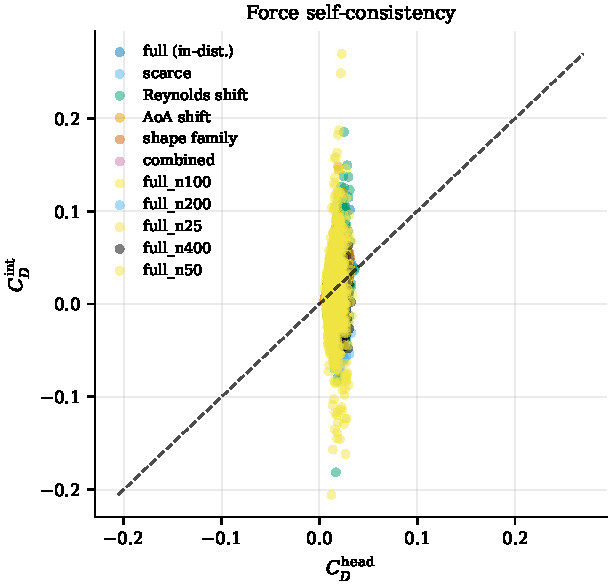
\includegraphics[width=0.7\textwidth]{figures/fig05_fsc_scatter.pdf}
  \caption{Force self-consistency: $\Cdint$ against $\Cdhead$, one point per
           test simulation pooled over all three models, coloured by split,
           against the identity line. Distance from the identity line is
           \FSC.}
  \label{fig:fsc_scatter}
\end{figure}

\begin{figure}[t]
  \centering
  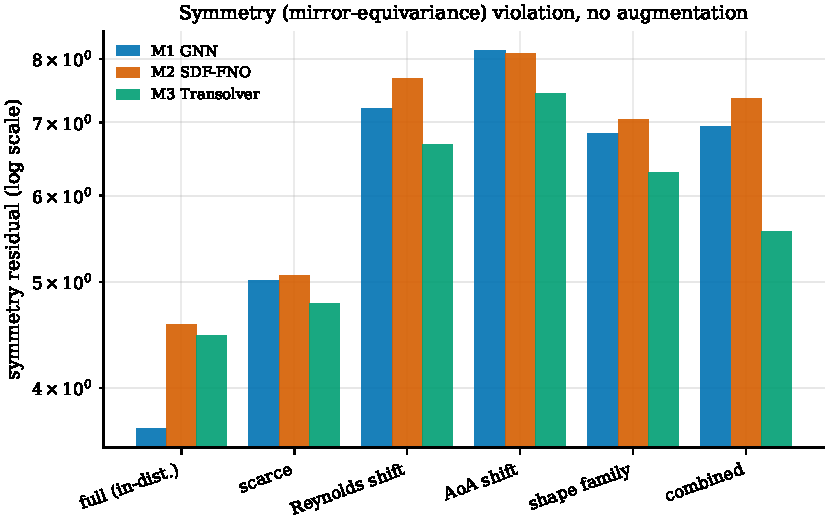
\includegraphics[width=0.75\textwidth]{figures/fig10_symmetry.pdf}
  \caption{Symmetry (mirror-equivariance) residual per model, by split, log
           scale; no augmentation is applied in any run reported here
           (\S\ref{sec:models}). The residual grows from \splitname{full} to
           \splitname{aoa} for every architecture and never approaches zero,
           confirming that none of the three encodings is built to be
           equivariant to reflection; \Mtrans{} is consistently the least
           violating of the three, \Mgnn{} and \Mfno{} track each other
           closely. The augmentation/loss ablation that would test whether
           this is trainable away is Table~\ref{tab:ablations}'s
           \Losssym{} row (pending, \S\ref{sec:results_ablations}).}
  \label{fig:symmetry}
\end{figure}

\subsection{Calibration}
\label{sec:results_calibration}

Table~\ref{tab:calibration} and Figures~\ref{fig:reliability}--\ref{fig:width_dists}
report split-conformal calibration of the integrated drag band $\Cdint$ at
nominal 80/90/95\%, matched (calibrate and test on the same split's own sets)
and transfer (calibrate on \splitname{full}, deploy on the shifted split).
Ensembles are $K=5$ for \Mfno{} and \Mtrans{} on \{\splitname{full},
\splitname{reynolds}, \splitname{aoa}, \splitname{shape5}\}; \Mgnn's ensembles
were still training on the cloud queue as this section was written, so every
\Mgnn{} row here is $K=1$ --- a single member, the \emph{absolute} nonconformity
score (a fixed interval half-width, not one that adapts to how hard a given
input is), not the input-adaptive \emph{normalized} score $K\geq3$ enables. That
distinction matters for reading the table: \Mgnn's coverage swings are what a
fixed-width band produces when calibration-set and test-set difficulty differ,
not a smooth degradation curve, and should not be over-interpreted as a
property of the graph encoder specifically until the $K\geq3$ row lands
(\S\ref{sec:results_ablations}/PLAN\_PHASE3.md \S3).

\textbf{In distribution, matched calibration is close to nominal for every
model}: \Cdint{} coverage at 90\% is $0.845$ (\Mgnn, $K{=}1$), $0.955$ (\Mfno),
$0.91$ (\Mtrans) --- the conformal guarantee behaving as designed when
calibration and test data are exchangeable. This is the sanity check, not the
finding.

\textbf{Under shift, coverage moves in both directions and the guarantee is not
reliable}, worst on the two flow-regime shifts. On \splitname{reynolds}, \Mgnn{}
collapses to $0.698$ at nominal 90\% (ECE $0.214$, a $\sim$10--20$\times$ jump
over its own in-distribution ECE of $0.045$); \Mfno{} and \Mtrans{} hold up
better under this shift ($0.895$ and $0.938$) but are not exempt from failure
elsewhere: \Mfno{} undercovers on \splitname{shape5} ($0.763$ at nominal 90,
ECE $0.12$, its worst split), the shift \S\ref{sec:results_ood} found mildest
for \emph{field accuracy} but not for calibration --- a reminder that these are
different failure modes measured on the same axis, not the same number twice.
\Mtrans{} is the most consistently calibrated of the three across every split
reported (coverage within $0.87$--$0.95$ of a 0.90 nominal target everywhere),
matching its position as the field-accuracy and (mostly) self-consistency
leader, but even it undercovers on \splitname{shape5} ($0.867$) rather than
holding exactly at nominal.

\textbf{Matched versus transfer calibration does not order cleanly.} Naively,
matched calibration should be the more defensible number (it uses that split's
own, in-principle-exchangeable calibration set) and transfer should be worse (it
reuses \splitname{full}'s calibration set on a distribution it was never fit
to). The data does not cooperate: on \splitname{reynolds}, transfer calibration
\emph{outcovers} matched for \Mgnn{} ($0.825$ vs.\ $0.698$) and for \Mfno{}
($0.942$ vs.\ $0.895$); on \splitname{shape5}, transfer beats matched for
\Mfno{} ($0.847$ vs.\ $0.763$) but loses to it for \Mgnn{} ($0.841$ vs.\
$0.945$, where matched \emph{overcovers}) and for \Mtrans{} ($0.814$ vs.\
$0.867$). No single choice of calibration set is reliably safer once
exchangeability has already broken; this is itself evidence that the failure is
structural (the score's relationship to error has genuinely changed under
shift) rather than a fixable artifact of which calibration set was used.

\textbf{Interval width widens under shift for every model (Figure~\ref{fig:width_dists}),
but under-compensates.} $\Cdint$ band width at nominal 90\% grows from
\splitname{full} to the harder splits --- e.g.\ \Mfno{} from $0.0085$ (full) to
$0.022$ (reynolds), \Mtrans{} from $0.0056$ to $0.021$ --- roughly $2.5$--$3.7\times$.
That the model's own uncertainty estimate grows at all under shift is
informative (an unresponsive score would be worse), but it is not enough:
coverage still drops on the same splits where width grows most, which is
exactly what "widening honestly but insufficiently" looks like in the reliability
diagram (Figure~\ref{fig:reliability}) as curves that bow away from the identity
line specifically on the OOD splits.

\textbf{The honest conclusion, stated as plainly as the numbers allow: split
conformal prediction repairs in-distribution calibration but its coverage
guarantee is not robust to distribution shift.} A 90\% conformal interval
computed on this study's splits must not be read as a 90\% probability
statement once the input has moved outside the calibration distribution ---
under a flow-regime shift (\splitname{reynolds}, \splitname{aoa}) that
probability can be as low as $0.70$ in this study, not $0.90$. Practically:
recalibrating on data from the deployment distribution, when any is available,
helps unpredictably rather than reliably (the matched-vs-transfer result
above), and the safer default for a practitioner is to treat any conformal
interval as calibrated only for inputs the acquisition/monitoring pipeline of
\S\ref{sec:activelearning} has confirmed are in-distribution.

On a calibration set of $n$ simulations disjoint from train and test, with
normalised nonconformity score
$\score_j = \abs{y_j - \ubar(\bx_j)} / (\sigmahat(\bx_j) + \eps)$ and $\qhat$ its
$\lceil (n+1)(\nomlevel) \rceil / n$ empirical quantile,
\begin{equation}
  \conf(\bx) = \left[ \ubar(\bx) - \qhat\,\sigmahat(\bx),\;
                      \ubar(\bx) + \qhat\,\sigmahat(\bx) \right],
\end{equation}
which satisfies $\Prob(y \in \conf(\bx)) \geq \nomlevel$ when calibration and
test data are exchangeable. Two granularities are calibrated separately:
per-simulation coefficient intervals, where the exchangeable unit is a whole
simulation and the guarantee is clean; and pointwise field intervals, where
points within a simulation are \emph{not} exchangeable, so we conformalise at the
simulation level with a quantile-over-points score and state the weaker
interpretation rather than implying a pointwise guarantee.

\begin{table}[t]
\centering
\caption{Split-conformal calibration of the integrated drag band ($C_D^{\mathrm{int}}$): empirical coverage, mean interval width and ECE. Matched calibrates on the split's own cal set; transfer (tr) calibrates on \texttt{full}'s cal.}
\label{tab:calibration}
\begin{tabular}{llrrrrrr}
\toprule
model & split & cov@.8 & cov@.9 & cov@.95 & cov@.9 (tr) & width@.9 & ECE \\
\midrule
M1 GNN & full (in-dist.) & 0.735 & 0.82 & 0.92 & 0.82 & 0.0332 & 0.0583 \\
M1 GNN & shape family & 0.718 & 0.863 & 0.959 & 0.818 & 0.0467 & 0.0426 \\
M1 GNN & Reynolds shift & 0.933 & 0.966 & 0.972 & 0.917 & 0.228 & 0.0737 \\
M1 GNN & AoA shift & 0.816 & 0.893 & 0.929 & 0.893 & 0.0575 & 0.015 \\
M2 SDF-FNO & full (in-dist.) & 0.885 & 0.955 & 0.98 & 0.955 & 0.00854 & 0.0567 \\
M2 SDF-FNO & shape family & 0.648 & 0.763 & 0.879 & 0.847 & 0.00731 & 0.12 \\
M2 SDF-FNO & Reynolds shift & 0.75 & 0.895 & 0.938 & 0.94 & 0.0218 & 0.0224 \\
M2 SDF-FNO & AoA shift & 0.913 & 0.944 & 0.974 & 0.929 & 0.0159 & 0.0605 \\
M3 Transolver & full (in-dist.) & 0.805 & 0.91 & 0.955 & 0.91 & 0.00562 & 0.00667 \\
M3 Transolver & shape family & 0.793 & 0.867 & 0.908 & 0.814 & 0.00746 & 0.0275 \\
M3 Transolver & Reynolds shift & 0.76 & 0.938 & 0.978 & 0.915 & 0.021 & 0.0351 \\
M3 Transolver & AoA shift & 0.821 & 0.949 & 0.959 & 0.949 & 0.0198 & 0.0265 \\
\bottomrule
\end{tabular}
\end{table}


\begin{figure}[t]
  \centering
  \begin{subfigure}{0.48\textwidth}\centering
    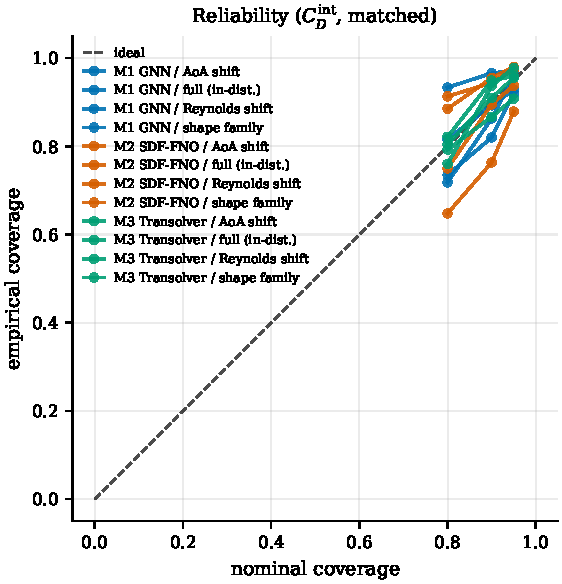
\includegraphics[width=\textwidth]{figures/fig06_reliability.pdf}
    \caption{Reliability.}\label{fig:reliability}
  \end{subfigure}\hfill
  \begin{subfigure}{0.48\textwidth}\centering
    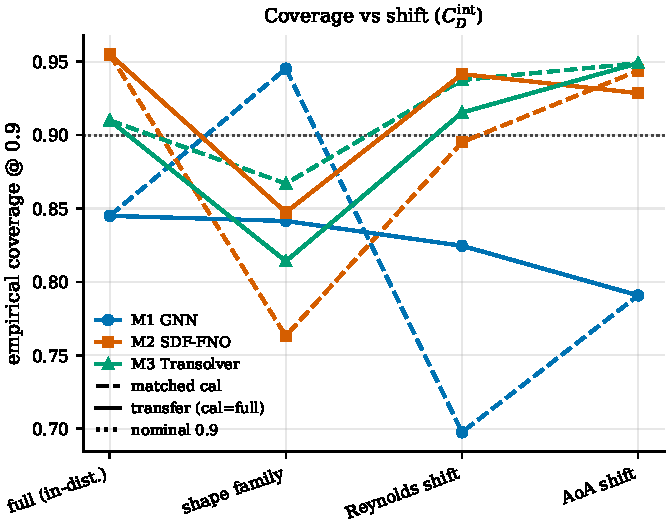
\includegraphics[width=\textwidth]{figures/fig07_coverage_vs_shift.pdf}
    \caption{Coverage versus shift.}\label{fig:coverage_vs_shift}
  \end{subfigure}
  \caption{Calibration in-distribution and under shift, largest available $K$
           per model ($K=5$ for \Mfno/\Mtrans, $K=1$ for \Mgnn): (a) empirical
           versus nominal coverage for the matched-calibration $\Cdint$ band;
           (b) empirical coverage at nominal 90\% against split, matched
           (dashed) versus transfer-calibrated on \splitname{full} (solid).}
  \label{fig:calibration}
\end{figure}

\begin{figure}[t]
  \centering
  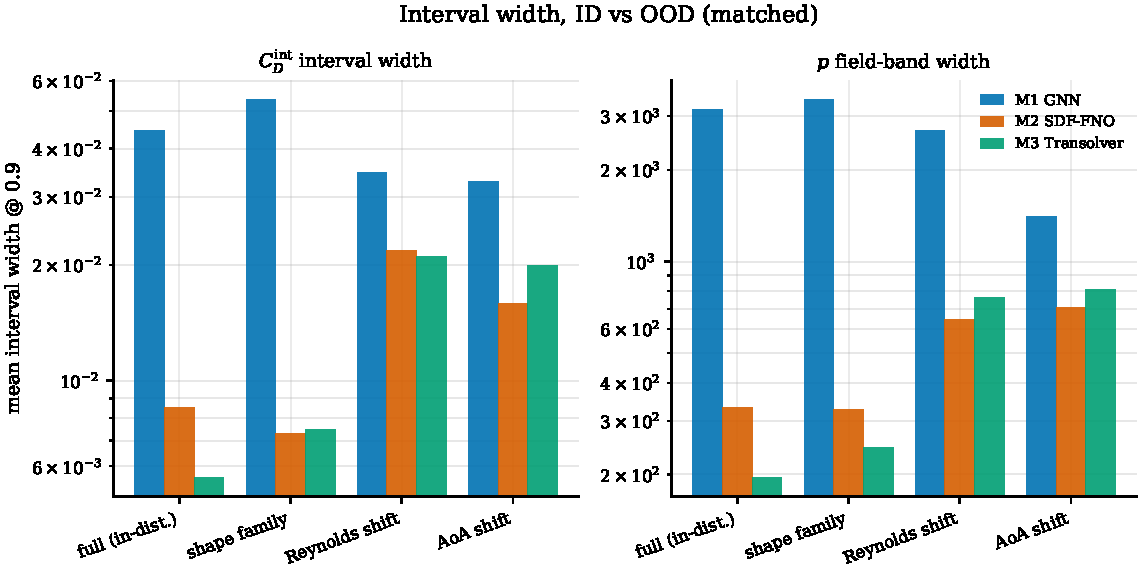
\includegraphics[width=0.9\textwidth]{figures/fig08_interval_width.pdf}
  \caption{Interval-width distributions, in-distribution versus OOD, matched
           calibration: mean interval width at nominal 90\%, per model and
           split, for the $\Cdint$ coefficient band and the pointwise field
           band (log scale). Widths grow from \splitname{full} outward for
           every model, but --- as Table~\ref{tab:calibration} and
           Figure~\ref{fig:coverage_vs_shift} show together --- not by enough
           to keep coverage at nominal under shift.}
  \label{fig:width_dists}
\end{figure}

\subsection{Data efficiency and cost}
\label{sec:results_efficiency}

\todo{The data-efficiency sweep (train sizes $\{25,50,100,200,400\}$, three
seeds, all three models, PLAN\_PHASE2.md Phase B) has not run yet --- Figure~9
below is a placeholder. Expect the transformer to need more data and the graph
baseline to hold up better when data is scarce; crossing curves would be a good
outcome, meaning method ranking depends on training budget and any
single-budget ranking (as in \S\ref{sec:results_id}--\ref{sec:results_ood}) is
under-specified.}

The cost side of Figure~\ref{fig:efficiency} does not need the sweep: measured
training wall-clock at the single 400-epoch, full-train budget already gives a
cost--accuracy Pareto plot (right panel). At that budget \Mgnn{} is
Pareto-\emph{dominated}: it costs \pending{3.0} GPU-h to train --- roughly
$7$--$8\times$ \Mfno's \pending{0.36}\,h or \Mtrans's \pending{0.41}\,h --- and
is also the least accurate of the three. The efficient frontier at this budget
is \Mtrans{} and \Mfno{}, at comparable, small training cost; \Mgnn's appeal
would have to come from some axis this study does not plot (implementation
simplicity, inference cost at deployment) rather than from the
training-cost/accuracy trade-off itself. Whether this ordering holds at smaller
training budgets is exactly what the data-efficiency sweep (left panel, still
pending) is designed to test.

\begin{figure}[t]
  \centering
  \begin{subfigure}{0.48\textwidth}\centering
    % 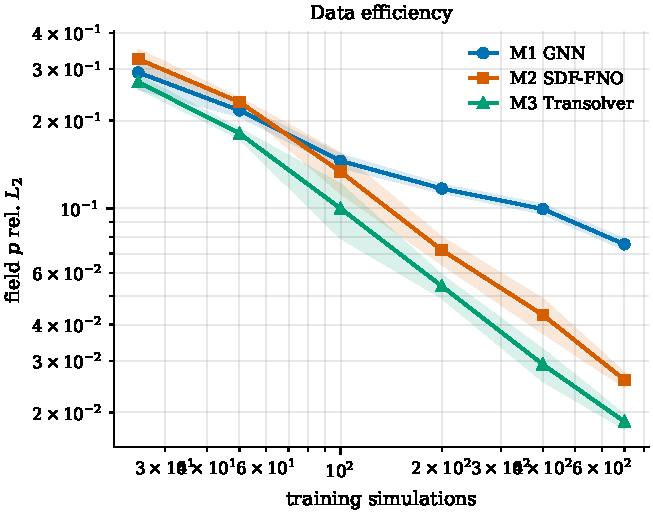
\includegraphics[width=\textwidth]{figures/fig09_data_efficiency.pdf}
    \figph[0.95\textwidth]{Figure 9. Data-efficiency curves, log-log, error
      against training-set size $\{25,50,100,200,400\}$ (+ 700/full, free from
      the core grid), seed bands shaded.}
    \caption{Data efficiency (pending).}\label{fig:data_efficiency}
  \end{subfigure}\hfill
  \begin{subfigure}{0.48\textwidth}\centering
    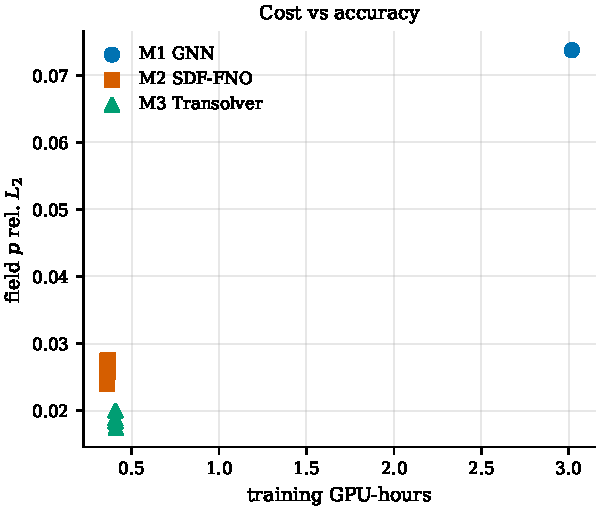
\includegraphics[width=\textwidth]{figures/fig12_cost_accuracy.pdf}
    \caption{Cost--accuracy at the full training budget (done).}\label{fig:pareto}
  \end{subfigure}
  \caption{Data efficiency and the cost--accuracy trade-off.}
  \label{fig:efficiency}
\end{figure}

\subsection{Ablations}
\label{sec:results_ablations}

\begin{table}[t]
  \centering
  \caption{\textbf{Table 4.} Ablations (lean v1 set): geometry encoding for
    \Mfno{} (SDF versus binary occupancy mask versus SDF plus normals),
    physics-loss weight $\lamF \in \{0, 1\}$, ensemble size
    $\nens \in \{1,3,5\}$ and conformal score choice (normalized versus
    absolute) --- both already computable from \texttt{results/uq}
    (\S\ref{sec:results_calibration}) but not yet tabulated here --- and
    field-aggregation choice (max versus quantile-0.9).}
  \label{tab:ablations}
  \begin{tabular}{llrrrr}
    \toprule
    Ablation & Setting & $\cp$ rel-$L_2$ & $\Cd$ MAE & \FSCrel & Coverage@90 \\
    \midrule
    \multicolumn{6}{c}{\itshape \todo{auto-generated}} \\
    \bottomrule
  \end{tabular}
\end{table}

% =====================================================================
\section{Active learning with solver verification}
\label{sec:activelearning}
% =====================================================================

This section turns \FSC{} and ensemble spread from diagnostics into a use: a
label-free score that picks which of many un-simulated candidates is worth the
cost of a new CFD run. The scoring half runs today on the existing \Mtrans{}
ensemble and needs no Fluent; the verification half --- actually running the
selected cases through an independent solver and checking whether the
"uncertain" ones really were harder --- is authored and ready but deferred
pending CPU availability (\S\ref{sec:discussion}), so this section reports the
selection honestly as a selection, not yet as a validated claim.

The pool is a parametric family of NACA 4- and 5-digit sections crossed with a
grid of $(\Rey, \aoa)$, none in the training set. Each candidate is scored
\begin{equation}
  \acq(\geom,\cond) = \underbrace{\sigmahat_{\Cd}(\geom,\cond)}_{\text{ensemble spread}}
    + \betaacq \underbrace{\FSC(\geom,\cond)}_{\text{self-inconsistency}}
    + \gammaacq \underbrace{\Losssym(\geom,\cond)}_{\text{symmetry violation}},
\end{equation}
all three normalised to unit variance over the pool, with
$\betaacq = \gammaacq = 1$ by default plus a sensitivity check. The top-$k$ are
selected subject to greedy farthest-point diversity in normalised design space,
so the selection cannot collapse onto $k$ near-duplicates. Baselines: random
selection and pure ensemble-variance selection.

\paragraph{The run.} Scorer \Mtrans{} at $K=5$ on \splitname{full}
(\texttt{transolver\_full\_k5}); pool of 630 candidates, NACA 4- and 5-digit
sections $\times$ $\Rey\in\{2,\dots,7\}\times10^6$ $\times$ $\aoa\in\{-6,0,6,12,18\}\degrees$,
every combination that coincides with a training case excluded (none did, by
construction of the grid); three arms of $k=8$ each (acquisition, ensemble
variance only, random). Figure~\ref{fig:active_learning}(a) plots the full pool
against $\aoa$, coloured by $\Rey$, with the three arms' selections marked; the
qualitative result is unambiguous before any Fluent run is needed: both
acquisition and pure-variance selection place all 8 of their picks at
$\aoa=18\degrees$, the top of the pool's angle grid and --- given the training
range in \S\ref{sec:data} tops out at $12.5\degrees$ --- comfortably into
post-stall territory at these Reynolds numbers, while the random arm spreads
across the whole envelope, including several low-angle, near-in-distribution
cases. Table~\ref{tab:fluent} lists the 8 acquisition-arm cases with their
ensemble spread, \FSC, symmetry residual and acquisition score.
Solver-verification status is exactly what the table's caption says: selected,
not yet verified.

\begin{table}[t]
\centering
\caption{\textbf{Table 5.} Active-learning acquisition-arm selection ($k=8$ of 630 pool candidates, scorer \texttt{transolver\_full\_k5}, $\beta=\gamma=1$): NACA section, Reynolds number, angle of attack, ensemble spread $\hat\sigma_{C_D}$, force self-consistency \FSC, symmetry residual $\Losssym$, and the resulting acquisition score. Generated from \texttt{results/active/selection\_summary.json} and \texttt{results/active/acquisition\_ranking.csv} (\S\ref{sec:activelearning}). \textbf{Selected, solver verification pending} (\S\ref{sec:activelearning}): the Fluent/surrogate comparison columns of the original design (Table~\ref{tab:datacard}-style CFD metadata) are added once \texttt{fluent/cases/} is executed.}
\label{tab:fluent}
\begin{tabular}{lrrrrrr}
\toprule
NACA section & $\mathrm{Re}$ & $\aoa$ (\si{\degree}) & $\hat\sigma_{C_D}$ & \FSC & $\Losssym$ & score $a$ \\
\midrule
0010 (4-digit) & $7\times10^6$ & 18 & 0.171 & 0.312 & 0.745 & 7.533 \\
2410 (4-digit) & $5\times10^6$ & 18 & 0.178 & 0.153 & 0.794 & 3.858 \\
4410 (4-digit) & $7\times10^6$ & 18 & 0.159 & 0.168 & 0.759 & 3.840 \\
0010 (4-digit) & $3\times10^6$ & 18 & 0.195 & 0.124 & 0.933 & 3.714 \\
33012 (5-digit) & $7\times10^6$ & 18 & 0.171 & 0.154 & 0.747 & 3.692 \\
4415 (4-digit) & $7\times10^6$ & 18 & 0.185 & 0.122 & 0.719 & 3.072 \\
0015 (4-digit) & $6\times10^6$ & 18 & 0.240 & 0.077 & 0.751 & 2.901 \\
24015 (5-digit) & $7\times10^6$ & 18 & 0.187 & 0.100 & 0.733 & 2.597 \\
\bottomrule
\end{tabular}
\end{table}


\paragraph{The falsifiable claim, restated precisely.} The claim this section
is designed to test is: \emph{cases with high acquisition score have higher
surrogate error, against the true (Fluent) solution, than randomly selected
ones.} That test needs the independent solver and cannot be run on the
surrogate's own training-data-derived truth without begging the question ---
computing "surrogate error" against AirfRANS would only confirm that the
acquisition score correlates with what it was built from. What \emph{can} be
said now, honestly, from the selection alone: the acquisition and
pure-variance arms agree with each other (all 8 vs.\ all 8 at
$\aoa=18\degrees$) and disagree sharply with random, which is the necessary
precondition for the falsifiable test to be informative --- if the arms had
picked statistically indistinguishable cases, no Fluent result could
discriminate them. Whether the harder-\emph{looking} cases are actually harder
in an independent solver is the open question \S\ref{sec:discussion} states as
a limitation, not a result.

\paragraph{Solver verification.}
Selected cases are run in Ansys Fluent: 2D steady incompressible RANS,
Spalart--Allmaras \citep{spalart1992sa} and $k$--$\omega$ SST
\citep{menter1994sst}, on parameterised C-grids with a documented $y^+$ target
and a three-level grid-independence study with GCI reported per
\citet{celik2008gci, roache1994perspective}.

\paragraph{The solver offset, and why it comes first.}
Our Fluent setup differs from the OpenFOAM setup behind AirfRANS in solver,
discretisation, mesh topology and convergence criteria. We therefore replicate
six AirfRANS \emph{test} simulations and measure the offset
$\shift_{\Cd} = \Cd^{\text{Fluent}} - \Cd^{\text{AirfRANS}}$ before interpreting
any surrogate-versus-Fluent gap. Without this, every disagreement is confounded.
\todo{Report the offset with its spread, and state whether the SA--SST spread
exceeds it --- if it does, that is the headline caveat.} The case list is
fixed and committed (\texttt{fluent/cases\_to\_run.json}): 3 grid-independence
replicates (\texttt{gridstudy\_naca0012\_re3e6\_a5}, levels 1--3) plus the 24
selected cases of the three arms above, 27 in total, rendered
(\texttt{fluent/make\_cases.py}) and ready to execute case-by-case per
\texttt{fluent/README.md}'s runbook the moment CPU is available. One risk is
worth flagging before any run, not after: every acquisition- and
variance-selected case sits at $\aoa=18\degrees$, and steady RANS convergence
at that angle, this close to and past stall, is not guaranteed --- a
non-converged case will be reported as such, not tuned to converge.

\begin{figure}[t]
  \centering
  \begin{subfigure}{0.48\textwidth}\centering
    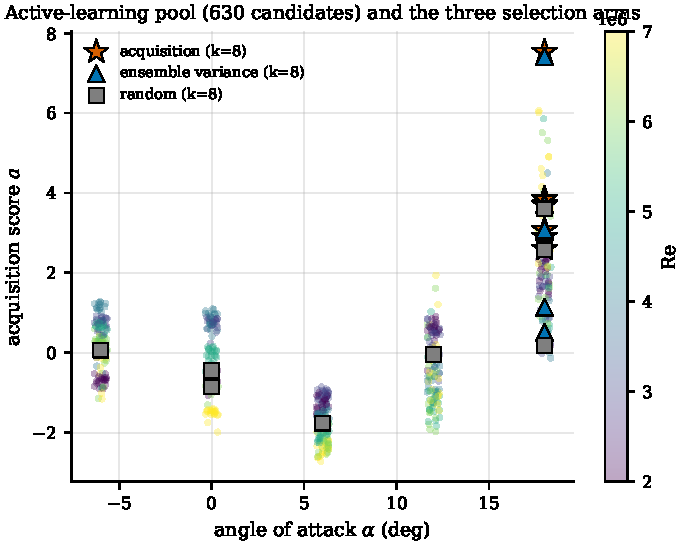
\includegraphics[width=\textwidth]{figures/fig11_active_pool.pdf}
    \caption{Pool and selections (done).}\label{fig:active_pool}
  \end{subfigure}\hfill
  \begin{subfigure}{0.48\textwidth}\centering
    \figph[0.95\textwidth]{Figure 11b. Surrogate error on Fluent-verified cases
      selected by acquisition score, by ensemble variance, and at random, with
      error bars that make the small sample size visually obvious rather than
      hiding it.}
    \caption{Verified error by arm (pending Fluent).}\label{fig:active_verify}
  \end{subfigure}
  \caption{Active learning: (a) the 630-candidate pool, coloured by $\Rey$,
           with the three $k{=}8$ arms marked --- acquisition and pure
           ensemble-variance selection agree with each other and disagree with
           random; (b) surrogate error on the Fluent-verified subset by
           selection strategy, the actual falsifiable test, pending CPU
           availability (\S\ref{sec:discussion}).}
  \label{fig:active_learning}
\end{figure}

% =====================================================================
\section{Discussion and limitations}
\label{sec:discussion}
% =====================================================================

Overclaiming is the single biggest risk to this paper's credibility, and this
section is the cheapest possible insurance against it. It is written to be
read, not skimmed.

\paragraph{Limitations.}
\begin{itemize}\itemsep2pt
  \item \textbf{Single seed on the core accuracy grid; ensembles are $K=5$ for
        two of three architectures, $K=1$ for the third, as reported here.}
        Every number in Tables~\ref{tab:indist}--\ref{tab:ood} and
        Figures~\ref{fig:error_vs_shift}--\ref{fig:fsc_scatter} is from one
        training run per (model, split) cell, seed 0 --- those headline
        field-error and $\Cd$-ranking gaps between architectures, some of
        which are only a few percentage points, are not yet accompanied by a
        seed-variance estimate at the core-grid level. The calibration study
        (\S\ref{sec:results_calibration}) does have that estimate for two of
        the three architectures: five-member deep ensembles (seeds 0--4) are
        complete for \Mfno{} and \Mtrans{} on \{\splitname{full},
        \splitname{reynolds}, \splitname{aoa}, \splitname{shape5}\}. \Mgnn's
        ensembles were still training on the cloud queue as this draft was
        written, so every \Mgnn{} calibration number here is $K=1$ (a single
        member, the fixed-width \emph{absolute} conformal score, not the
        input-adaptive \emph{normalized} one $K\geq3$ enables) --- read
        \Mgnn's calibration row as preliminary and the other two as backed by
        a real ensemble. The cross-split and cross-shift patterns, an order of
        magnitude larger than the between-architecture gaps, are far less
        likely to be single-seed noise, but core-grid seed variance is not
        the number that would let a reader check that directly.
  \item \textbf{One dataset family, and 2D only, in the results reported here.}
        Everything in this preprint is AirfRANS: 2D airfoils, incompressible
        RANS, one turbulence model (Spalart--Allmaras), one solver family
        (OpenFOAM, upstream). DrivAerNet++ (3D cars) is this project's
        designated extension but requires an interactive data-access step
        outside the current scope and contributes zero results here; no claim
        in this paper should be read as extending to 3D geometry, compressible
        flow, or any solver other than the one AirfRANS was generated with.
  \item \textbf{The Fluent verification set has not been run yet.} The
        acquisition pipeline, journal templates and the full 27-case list
        (\texttt{fluent/cases\_to\_run.json}: 3 grid-independence replicates
        plus the 24 selected cases of \S\ref{sec:activelearning}) are authored,
        rendered and checked, but the CFD runs themselves are deferred pending
        compute availability; \S\ref{sec:activelearning} reports what is
        selected and ready to run, not a completed external check. All 8
        acquisition-arm cases sit at $\aoa=18\degrees$
        (Table~\ref{tab:fluent}), which is both the reason the arm is
        informative (it disagrees sharply with random) and a convergence risk
        for steady RANS this close to stall; a non-converged case will be
        reported as such. When run, this is 24 selection cases plus a
        three-level grid-independence study --- a qualitative external check
        against 24 points, not a large-sample statistical test, and described
        that way throughout.
  \item \textbf{Reimplementations, not the authors' code.} All three
        architectures are reimplemented from the cited papers rather than run
        from the authors' released code (\S\ref{sec:models}), for a hardware
        dependency reason stated there. Absolute numbers are therefore not
        comparable with published ones; only the within-study comparison,
        which is matched by construction (parameter count, loss, optimiser,
        schedule, batch size, epoch budget), is meaningful.
  \item \textbf{Compute budget.} A single consumer GPU throughout: a 4\,GB
        Pascal-generation card locally, moved to a cloud Tesla T4 (16\,GB) once
        the study outgrew the local card, both fp32, no mixed precision. Every
        model trains for exactly 400 epochs at batch size 16
        (\S\ref{sec:models}); rankings under a substantially larger compute or
        parameter budget may differ, which the (currently pending) data-efficiency
        curves of Figure~\ref{fig:data_efficiency} are designed to expose
        rather than hide.
  \item \textbf{Conformal guarantees are exchangeability-conditional, and the
        measured breakage is a small-sample estimate.} The calibration study
        (\S\ref{sec:results_calibration}) is complete and reports realised
        coverage rather than assuming the nominal guarantee survives shift
        \citep{tibshirani2019covariateshift} --- under shape-family and
        flow-regime shift, exchangeability fails by construction, and coverage
        moves accordingly (as low as $0.70$ at a nominal 90\% on
        \splitname{reynolds}). Each split's coverage point is itself an
        empirical rate over that split's own test set ($n=196$--$511$,
        Table~\ref{tab:datacard}), not a large-sample asymptotic result, so the
        exact coverage numbers in Table~\ref{tab:calibration} carry their own
        (unreported here) sampling uncertainty on top of the qualitative
        finding that the guarantee degrades under shift.
  \item \textbf{The angle-of-attack pre-stall/post-stall breakout is not yet
        computed.} \S\ref{sec:results_ood}'s reading of the \splitname{aoa}
        result as a regime-crossing failure rests on the aggregate split
        number and domain knowledge about where these sections stall, not on
        a per-simulation separation indicator; that breakout
        (\S\ref{sec:data}) would make the claim precise.
  \item \textbf{Single author.} No co-author caught bugs. Mitigations: the
        force integrator is gated against ground truth before anything
        downstream runs (\S\ref{sec:protocol}), split disjointness is asserted
        programmatically for every manifest, three independent automated
        review passes audited the codebase before any GPU-hours were spent on
        results reported here and caught two real defects (a test-statistic
        leak into per-split normalisation, since fixed, and a stale-geometry
        bug in the symmetry check, since fixed), and \todo{name the human CFD
        and ML reviewers who read this}.
\end{itemize}

\paragraph{Negative and mixed results, reported as found.} The ridge baseline
--- 29 parameters, linear in shape and flow parameters, zero training cost ---
is competitive on $\Cd$ rank correlation across every split
($\rho_s\in[0.83,0.90]$, \S\ref{sec:results_id}--\ref{sec:results_ood}),
uncomfortably close to $\sim$1.3\,M-parameter neural operators trained for
hundreds of GPU-hours combined. The architecture that wins on field accuracy is
not always the architecture that is most internally self-consistent: on the two
hardest single-axis shifts, \Mfno{} out-consistents the field-accuracy leader
\Mtrans{} (\S\ref{sec:results_consistency}). All three architectures carry a
large, roughly uniform symmetry residual with no augmentation applied
(\S\ref{sec:results_id}, Figure~\ref{fig:symmetry}) that \emph{grows} under
shift for every model rather than staying fixed; whether augmentation removes
it is an open ablation, not yet run. Matched-versus-transfer conformal
calibration (\S\ref{sec:results_calibration}) does not order cleanly either:
naively, calibrating on a split's own data should be the safer choice, but
transfer calibration from \splitname{full} beats matched calibration for
\Mgnn{} and \Mfno{} on \splitname{reynolds} and for \Mfno{} on
\splitname{shape5} --- a genuinely mixed result, reported as found rather than
rounded into "matched is always better." \todo{Whichever of these also hold
once the remaining phases land, report them too: physics losses that only
shrink the residual they penalise; symmetry augmentation that fixes the
symmetry residual and nothing else; whether the acquisition-selected cases
(concentrated at $\aoa=18\degrees$, \S\ref{sec:activelearning}) turn out no
harder than random once Fluent-verified --- a null result there is a real
finding and must be printed as willingly as a positive one.}

% =====================================================================
\section{Conclusion}
\label{sec:conclusion}
% =====================================================================

This paper's contribution is a measurement protocol, not a leaderboard
position, and the three architectures audited under it earn that framing: on
raw field accuracy they separate cleanly (\Mtrans{} $>$ \Mfno{} $>$ \Mgnn,
everywhere, by up to $4\times$), but on the quantity a designer actually
conditions a decision on --- $C_D$ rank correlation --- they are within a few
parts per thousand of each other and only modestly ahead of a 29-parameter
ridge baseline. A field-error leaderboard, run in isolation, would have
reported a result that barely survives contact with the metric a wing or hull
designer would use. That is the paper's first and most transferable finding:
\emph{for down-selection tasks, measure the ranking metric, not only the field
norm, before declaring an architecture the winner.}

The second finding is that self-consistency and calibration are not
by-products of accuracy --- they have to be measured separately, and they
disagree with the accuracy ranking often enough to matter. \Mfno{} out-consistents
the field-accuracy leader \Mtrans{} on the two hardest single-axis shifts
(\S\ref{sec:results_consistency}); split-conformal coverage, backed by a real
$K=5$ ensemble for two of the three architectures, holds at its nominal level
in distribution and degrades unevenly under shift, worst on the flow-regime
axes (\S\ref{sec:results_calibration}) where field error also degrades most ---
but the two degradations are not the same number, and a model can be the most
accurate in distribution while being neither the most self-consistent nor the
best calibrated once conditions shift.

The third finding is architectural rather than about any one model: every
axis this protocol measures --- field error, $C_D$ ranking, \FSC, symmetry
residual, conformal coverage --- degrades sharply on the two shifts that cross
into a new flow regime (\splitname{reynolds}, \splitname{aoa}) and only mildly
on the shift that stays inside the training regime (\splitname{shape5}, a new
NACA digit family at the same Reynolds and angle of attack), even though
\splitname{shape5} carries the largest raw shift magnitude
$\shift$ by construction (\S\ref{sec:protocol}). These models interpolate
within a flow regime and do not extrapolate across one, and a
design-space-distance heuristic does not see that difference; \FSC{} and
ensemble spread, both label-free, do a better job of flagging it, which is
what makes them usable inside the acquisition loop of
\S\ref{sec:activelearning}.

\paragraph{What a practitioner should do differently on Monday morning.} Report
the ranking metric alongside the field norm before claiming an architecture
win, especially for a design task. Compute \FSC{} on every prediction a
surrogate makes, including in production on shapes with no ground truth --- it
is free, it needs no label, and this study's own numbers show it tracks
distribution shift at least as sensitively as field error. Treat a conformal
interval as calibrated only for inputs confirmed in-distribution by that same
label-free check, not as a blanket probability statement; recalibrating on
deployment data is not a reliable fix on its own (\S\ref{sec:results_calibration}'s
matched-versus-transfer result). And when deciding where to spend the next
expensive simulation, an ensemble-and-consistency acquisition score is cheap
to compute and, in this study's pool, concentrates its picks exactly where
domain knowledge says a RANS surrogate should be least trusted --- a start
worth solver-verifying, which is this paper's own next step.

% =====================================================================
\section*{Reproducibility statement}
% =====================================================================
Code is released under the MIT licence at \todo{repository URL}; a Zenodo DOI
is minted at public release, alongside a rules-compliant public staging copy of
the repository (the working repository is private during the study for
scooping-risk reasons, per the project's own decision log, and is restructured
into the public layout only once, not iteratively). The release includes:
split-ID manifests for all six splits (\texttt{data/splits/*.json}, the exact
train/calibration/test simulation lists each result in this paper was produced
from); per-run configs and metrics
(\texttt{results/<run\_id>/\{config.yaml,metrics.json,per\_sim.csv\}} for every
core, ensemble and baseline run); the conformal calibration reports
(\texttt{results/uq/*.json}) Table~\ref{tab:calibration} and
Figures~\ref{fig:reliability}--\ref{fig:width_dists} are generated from; the
active-learning pool, scores and selection
(\texttt{results/active/*}, \texttt{fluent/cases\_to\_run.json}); and, once
solver-verified, the Fluent case set itself (meshes, journals, convergence
histories, extracted surface data). Every figure and table in this paper is
produced by \texttt{scripts/make\_figures.py} / \texttt{scripts/make\_tables.py}
from the committed JSON, not hand-typed, so a reader can regenerate every
number from the release.

Data: AirfRANS \citep{bonnet2022airfrans} is licensed ODbL-1.0
(attribution and share-alike on derived databases); this release publishes
split manifests and code, never a processed copy of the AirfRANS fields, and
respects the share-alike obligation on any derived database. DrivAerNet++
\citep{elrefaie2024drivaernetpp}, licensed CC~BY-NC-4.0, contributes zero
results to this preprint (\S\ref{sec:data}) and is not included in the release.

Reimplementation note (\S\ref{sec:models}): \Mgnn, \Mfno{} and \Mtrans{} are
each reimplemented from the cited papers, not run from the authors' released
code, for the hardware-dependency reason stated in \S\ref{sec:models}. No
number in this paper should be read as a reproduction of a published result;
the meaningful comparison is the within-study one, matched by construction
across all three families (parameter count, loss, optimiser, schedule, batch
size, epoch budget).

Normalisation (\S\ref{sec:models}): every split's input/output statistics are
computed from that split's own training list only, never from a shared global
set and never from that split's calibration or test data, so no OOD split's
test statistics can leak into training even indirectly through input scaling
--- this is a deliberate fix to an earlier version of the pipeline that shared
one global normalisation across splits, described honestly here because it
changed reported OOD numbers (the corrected numbers are what this paper
reports; the affected runs were retrained under the fix before any result in
this paper was produced).

Seeds: every run records its seed in \texttt{metrics.json}; deep-ensemble
members are seeds 0--4 (or 0 alone where noted); training is deterministic
given seed, split manifest and code commit, modulo the floating-point
non-associativity inherent to GPU reduction order, which is not controlled for
across the local Quadro P2000 and the cloud Tesla T4 (\S\ref{sec:discussion}).

\section*{Acknowledgements}
\todo{Reviewers, compute, dataset authors.}

\bibliography{refs}

\appendix

% =====================================================================
\section{Hyperparameters and training details}
\label{app:hyper}
% =====================================================================
Full configs are committed at \texttt{configs/\{gnn,sdf\_fno,transolver\}.yaml}
and, per run, at \texttt{results/<run\_id>/config.yaml}; this appendix
reproduces the values needed to rebuild a run without opening those files.

\begin{table}[h]
  \centering
  \caption{Architecture hyperparameters, one column per model.}
  \label{tab:app_arch}
  \begin{tabular}{lccc}
    \toprule
    & \Mgnn & \Mfno & \Mtrans \\
    \midrule
    encoder width / channel dim         & 128 (hidden)      & 32 (FNO width)     & 128 ($d$) \\
    depth                               & 8 (msg.\ rounds)  & 4 (FNO layers)     & 4 (attn.\ layers) \\
    geometry parameter                  & $k=16$ (kNN)      & 16 modes, $64{\times}64$ grid & $M=32$ slices \\
    conditioning                        & pos./normal/curvature & signed distance ($\sdf$) & 8 heads, slice attn. \\
    grouped/spectral detail             & --                & 4 spectral groups; kernel enc/dec $k{=}8$ & --- \\
    positional Fourier frequencies      & 6                 & 6                  & 6 \\
    coefficient head                    & \multicolumn{3}{c}{trunk 128--256, 2-layer MLP, deep-set mean+max pooling (identical across models)} \\
    parameter count                     & 1{,}389{,}637     & 1{,}373{,}605      & 1{,}281{,}701 \\
    \bottomrule
  \end{tabular}
\end{table}

\begin{table}[h]
  \centering
  \caption{Training hyperparameters, matched across all three architectures
    (\S\ref{sec:models}) and identical in every core-grid, ensemble and
    baseline-comparable run.}
  \label{tab:app_train}
  \begin{tabular}{ll}
    \toprule
    Optimiser & Adam, weight decay 0 \\
    Learning rate & $10^{-3}$ initial, cosine schedule to $10^{-6}$, 0 warmup epochs \\
    Gradient clipping & global norm 1.0 \\
    Batch size & 16 (all three architectures) \\
    Epochs & 400 \\
    Precision & fp32 (no AMP; Pascal-generation local GPU has no practical fp16 path) \\
    Loss weights (default) & $\lambda_H=0.1$ (coefficient head, always on); $\lamF=\lamB=\lamS=\lamD=0$ \\
    Seeds & core grid: 0; deep ensembles: 0--4 (\Mfno/\Mtrans, $K=5$) or 0 (\Mgnn, $K=1$ as reported) \\
    Normalisation & per-split, train-list-only statistics (\S\ref{sec:models}) \\
    Checkpointing & every epoch, resumable from the last checkpoint \\
    \bottomrule
  \end{tabular}
\end{table}

% =====================================================================
\section{CFD setup and grid-independence study}
\label{app:cfd}
% =====================================================================
The design in this appendix is complete and frozen (\texttt{docs/FLUENT\_PLAN.md});
the measured values below are \todo{pending} until the CPU-gated runs of
\S\ref{sec:activelearning} execute. Written for a CFD reviewer, who reads this
appendix first.

\paragraph{Meshing.} \texttt{fluent/mesh\_gen.py} writes the C-grid mesh
directly as a native Fluent \texttt{.msh} from the NACA parametric equations,
rather than through a general-purpose mesher (gmsh cannot emit Fluent's format
at all; \texttt{meshio}'s Fluent writer drops boundary zones): the topology is
a single structured block with a known index map, so there is nothing for a
mesher to discover, and the $y^+$ target and the grid-independence refinement
ratio become exact one-line parameters instead of sizing-function requests
that are only approximately honoured. \texttt{mesh\_gen.py --self-check}
re-parses the written mesh and asserts index ranges, owner/neighbour
consistency and non-degenerate faces; \texttt{fluent/templates/mesh\_cgrid.rpl}
is an independent ICEM Tcl cross-check kept as a fallback, not exercised in
this preprint.

\paragraph{Solver setup.} 2D steady incompressible RANS, two turbulence
closures run per case for a spread estimate: Spalart--Allmaras
\citep{spalart1992sa} (matching AirfRANS's own OpenFOAM setup) and
$k$--$\omega$ SST \citep{menter1994sst}. $y^+$ target and first-cell height:
\todo{value, from the flat-plate correlation in FLUENT\_PLAN.md \S3}.

\paragraph{Grid-independence study.} Three refinement levels per case
(\texttt{gridstudy\_naca0012\_re3e6\_a5\_L\{1,2,3\}}, already in
\texttt{fluent/cases\_to\_run.json}), apparent order $p$ and GCI computed per
\citet{celik2008gci, roache1994perspective}: \todo{apparent order $p$, GCI on
the fine-grid solution, mesh quality metrics per level}.

\paragraph{Solver offset against AirfRANS.} Six AirfRANS test simulations
replicated in Fluent to measure $\shift_{\Cd} = \Cd^{\text{Fluent}} -
\Cd^{\text{AirfRANS}}$ before any surrogate-versus-Fluent comparison is
interpreted (\S\ref{sec:activelearning}): \todo{offset with spread; whether
the SA--SST spread exceeds the offset itself, the headline caveat if so; $\cp$/
$c_f$ overlays localising where the two setups disagree}.

\paragraph{Acceptance criteria.} A case counts only if it meets the RUNBOOK's
convergence criteria (\texttt{fluent/README.md}); a case that does not
converge --- a real risk at $\aoa=18\degrees$, where every acquisition-arm
selection sits (\S\ref{sec:activelearning}) --- is reported as non-converged,
not tuned until it converges.

% =====================================================================
\section{Additional figures}
\label{app:figures}
% =====================================================================
\todo{Per-split $\cp$ and $\tauw$ profiles, per-model residual histories,
additional reliability diagrams, the acquisition-score sensitivity check over
$\betaacq$ and $\gammaacq$.}

% =====================================================================
\section{Compute accounting}
\label{app:compute}
% =====================================================================
Every number below is summed directly from \texttt{train\_time\_s} across the
50 committed \texttt{results/<run\_id>/metrics.json} files that carry it as of
this draft (core grid plus every committed deep-ensemble member; the two
non-learned baselines and one run recorded without a timing field are
excluded from the sum, not from the study); it is therefore a lower bound on
total compute spent, not an estimate: sessions that
were retrained from scratch after an infrastructure bug (a mount-path
assumption that broke cross-session resume, \S\ref{sec:discussion}) are not
separately itemised because their wall-clock is already folded into whichever
completed run superseded them, and GNN-ensemble sessions still in flight on
the cloud queue at time of writing are not yet in this sum.

\begin{table}[h]
  \centering
  \caption{Training compute, summed over every committed run
    (core grid + deep-ensemble members), by model.}
  \label{tab:app_compute}
  \begin{tabular}{lrr}
    \toprule
    Model & GPU-hours & \# runs summed \\
    \midrule
    \Mgnn{}      & 10.45 & 6  \\
    \Mfno{}      & 6.08  & 22 \\
    \Mtrans{}    & 6.74  & 22 \\
    \midrule
    Total (neural)  & 23.27 & 50 \\
    \bottomrule
  \end{tabular}
\end{table}

\Mgnn{} costs more per run despite having the fewest runs summed
(kNN reconstruction on every forward pass is the dominant cost, matching
\S\ref{sec:results_efficiency}'s single-run measurement of $\sim$3\,\si{\hour}
for one \Mgnn{} \splitname{full} run against \Mfno's 0.36 and \Mtrans's
0.41\,\si{\hour}); \Mfno{} and \Mtrans{} sum more GPU-hours in this table only
because more of their ensemble members (five seeds on four splits each) had
landed locally at draft time. Baselines (ridge, constant) are not trained in
the gradient-descent sense and are excluded (fit cost is sub-second CPU).
Hardware: local gating and development on a Quadro P2000 (4\,GB, Pascal,
CPU-bound for anything beyond a smoke test); all runs summed above trained on
Kaggle's free-tier Tesla T4 (16\,GB), chained across $\sim$11-hour sessions
(\S\ref{sec:models}, \S\ref{sec:discussion}); the local machine's CPU was never
used for training. Energy accounting is not available from the Kaggle API and
is not reported.

\end{document}
